\documentclass{beamer}

\usefonttheme[onlymath]{serif}

\usetheme[pageofpages=of,% String used between the current page and the
                         % total page count.
          bullet=circle,% Use circles instead of squares for bullets.
          titleline=true,% Show a line below the frame title.
          alternativetitlepage=true,% Use the fancy title page.
          titlepagelogo=logo-polimi,% Logo for the first page.
          ]{Torino}
          
%          watermark=watermark-polito,% Watermark used in every page.
%          watermarkheight=100px,% Height of the watermark.
%          watermarkheightmult=4,% The watermark image is 4 times bigger
%                                % than watermarkheight.

%\usepackage[margin=0.7in]{geometry}
\usepackage[latin1]{inputenc}
\usepackage[english]{babel}
\usepackage{amsmath}
\usepackage{subfig}
\usepackage{booktabs}
\usepackage{wrapfig}
%\usepackage{cases}
%\usepackage[makeroom]{cancel}
%\usepackage{amsmath,tabu}
%\usepackage[fleqn]{mathtools}
%\usepackage[fleqn]{amsmath}
%\usepackage{bm}
%\usepackage{tikz}
%\usepackage{enumitem}
%\usepackage{wrapfig}
%\usepackage{graphicx}
\usepackage{siunitx}
%\usepackage{microtype}
%\usepackage{array,tabularx}
%\usepackage{float}
%\usepackage{booktabs}
%\usepackage{import}
%\usepackage{cases}
%\usepackage{graphicx,subfigure}
\usepackage{myUnitOfMeasure}
%\usepackage{myThermodynamics}
\usepackage{myMath}
%\usepackage{mathtools}
%\usepackage{gensymb}
\usepackage{xcolor}


\newcommand{\myspace}[0]{\vspace{0.3cm}}
\newcommand{\myspaceneg}[0]{\vspace{-0.15cm}}
\newcommand{\dmid}{D_\text{mid}}
\newcommand{\highlightgreenA}[1]{\textcolor{chameleongreen1}{#1}}
\newcommand{\highlightgreenB}[1]{\textcolor{chameleongreen2}{#1}}
\newcommand{\highlightgreenC}[1]{\textcolor{chameleongreen3}{#1}}% best
\newcommand{\highlightgreenD}[1]{\textcolor{chameleongreen4}{#1}}

\author{Rossi Andrea}
\title{Preliminary design of a High Pressure Steam Turbine}
\institute{Politecnico di Milano}
\date{}

\begin{document}


\begin{frame}[t,plain]
\titlepage
\end{frame}

\begin{frame}[t]{The design specifications}
The project consist in the preliminary design of the \highlightgreenC{\emph{high pressure}} part of a steam turbine.

The design process requires some initial data other than many other assumptions.

Inlet flow characteristics, in terms of total quantities, are:
\begin{itemize}
	\item ${p}_{T} = 150\,\text{bar}$
	\item $T_{T} = 700\celsius$
\end{itemize}
The stages must provide a pressure ratio $\beta$ of 2.5.

Since the first stage of the design is the first stage of the whole machine, the \textbf{inlet} direction is assumed to be purely \emph{\textbf{axial}}.
\end{frame}

\begin{frame}[t]{The model of the fluid}
The text leave the choice of the \textbf{model of the fluid} to our responsibility.
The two main alternatives are:
\begin{itemize}
	\item perfect gas with $\gamma = 1.33$ and constant $\text{c}_\text{p}$;
	\item steam tables;
\end{itemize}
Since steam tables are available as an additional library in Matlab, to guarantee a better precision they are used.

In particular the library \textbf{XSteam} is applied in any calculation of steam properties.
\end{frame}

\begin{frame}[t]{The design process}
Most of the choices related to the machine are taken based \textbf{not only} on common techniques like \emph{loading criteria}, but also on the comparison of the result from the implementation of the model in computer code.

\myspace
The machine will be implemented in a power plant, so the first goal of the design is
\begin{center}
\highlightgreenC{\textbf{highest efficiency as possible}}
\end{center}
\end{frame}

\begin{frame}[t]{The model of the machine - The inputs}
The data available from the costumer are necessary but not sufficient.

So as additional and more specific input for our model we take:
\begin{itemize}
	\item the reaction degree in the middle diameter $\chi$,
	\item the rotational speed $n$ in $\text{rpm}$,
	\item the number of stages,
	\item the flow coefficient $\phi = {v}_{a} / U$,
	\item the minimum value of blade height over the diameter $\text{b} / \dmid$,
	\item the partial admission coefficient $\varepsilon$,
	\item the solidity $\sigma = \text{chord} / \text{pitch}$
	\item the ratio of the chord over the blade height
\end{itemize}
\end{frame}

\begin{frame}[t]{The model of the machine - The inputs}
\begin{itemize}
	\item the blade thickness over the chord
	\item the absolute clearance
	\item the number of seals per rotor
	\item an initial guess of the efficiency ($\eta = 1$ could be a guess)
	\item the number of section in which divide the span
	\item other numerical and computational parameters
		\begin{itemize}
			\item the maximum number of iterations;
			\item the tolerances ($1\E{-6}$).
		\end{itemize}
\end{itemize}
\end{frame}

\begin{frame}[t]{The model of the machine - The inputs}

Some of the input are trivial and mandatory, but other are chosen.

\myspace
For example the \textbf{\emph{number of stages}} is taken as input but it could also be the result of the calculation. 

In fact the alternative was to choose the \emph{work coefficient} $\lambda = l / U^2$, and in that case the number of stages would have been the result.

\myspace
Since the number of stages is a very significant parameter respect to the work coefficient this choice has been made.

\myspace
Another parameter is the \emph{flow coefficient} that can be replaced with $k_p = U / v_1$
\end{frame}

\begin{frame}[t]{The model of the machine - The main loop}
The whole process requires the total efficiency of the machine. 

The efficiency is also an output of the design: $\Rightarrow$ \textbf{iterative loop}.

\begin{figure}[hbtp]
\centering
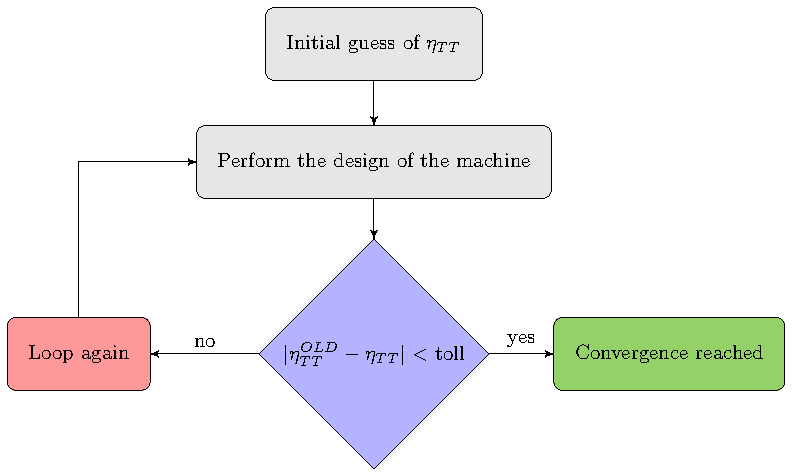
\includegraphics[scale=0.7]{fig/mainloop_fig.pdf}
\end{figure}

\end{frame}



\begin{frame}[t]{The model of the machine - The main loop}
At the beginning we only have the total enthalpy at the inlet.
\begin{equation}
h_T^{0} = h(p_{T_{0}}, \text{T}_{T_{0}})
\end{equation}
To compute the isoentropic outlet enthalpy we have simply to consider that 
the initial final entropy are the same by definition.
\begin{equation}
s_0 = s_{T_{0}} = s(p_{T_{0}}, \text{T}_{T_{0}})
\end{equation}
\begin{equation}
h_{T_\text{isoentropic}}^{\text{end}} = h\left(\dfrac{p_{T_{0}}}{\beta_{TT}}, s_{0}\right)
\end{equation}
Finally we calculate the outlet enthalpy from the efficiency:
\begin{equation}
h_{T}^{\text{end}} = h_T^{0} - \eta_{TT} \cdot (h_{T_{0}} - h_{T_\text{is}}^{\text{end}})
\end{equation}
\end{frame}



\begin{frame}[t]{The model of the machine - The main loop}
Dividing the enthalpy drop by the stages number we find the enthalpy drop of the single stage that is also the \emph{Euler work} of the stage.
\myspaceneg
\begin{equation}
l_{eu} = u \cdot \left( v_{1T} - v_{2T} \right) = \dfrac{h_T^{0} - h_{T}^{\text{end}}}{\text{N}_{\text{stages}}}
\end{equation}

The first quantity in which we are interested is the peripheral speed $\text{U}$. We can obtain it from the mass flow rate:
\myspaceneg
\begin{equation}
\label{eq:mdot_U}
\dot{m} = \rho_0\footnote{ \raggedleft The static density is unknown but since we are iterating we keep the total one as first guess ad we update it at every cycle} \cdot v_A \cdot S = \rho_0 \cdot v_A \cdot \pi \, \left(\dfrac{b}{\dmid}\right) \, \dmid^2
\end{equation}
Having defined both $\phi = v_A / \text{U}$ and $\dmid = 60 / (2\, \pi \, n) \, \text{U}$ the mass flow rate is only function of the the cube of the peripheral speed.
\end{frame}

\begin{frame}[t]{The model of the machine - The velocity triangle}
To design the velocity triangle we have to make some choices:
\begin{itemize}
	\item repeated stage, so $v_0 = v_2$
	\item constant axial velocity $v_{0A} = v_{1A} = v_{2A} = v_A$
	\item the first stator has an axial inlet so it can break the repeated stage rule. In this case its velocity will be $v_0 = v_A$
\end{itemize}
Now what we need are:
\begin{itemize}
	\item $\text{U}$ previously found from equation \ref{eq:mdot_U};
	\item $v_A = \phi \cdot \text{U}$
	\item $v_{1T} - v_{2T} = \Delta v_T = -\dfrac{l}{\text{U}}$
	\item $v_{1T} + v_{2T} = 2\, \text{U} \cdot \left( 1 - \chi_{\text{mid}} \right)$
\end{itemize}
\end{frame}

\begin{frame}[t]{The model of the machine - The velocity triangle}
As we can see in figure \ref{fig:velocitytriangle_example} the outlet velocity of the stage is almost but not exactly axial.

The \textbf{first stage} will have a reaction degree at midspan slightly different from the desired. 

\begin{figure}[hbtp]
\centering
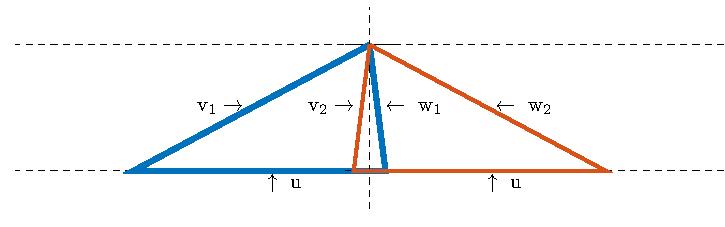
\includegraphics[scale=0.7]{fig/velocity_triangle_example.pdf}
\caption{Example of result of a velocity triangle}
\label{fig:velocitytriangle_example}
\end{figure}
\end{frame}


\begin{frame}[t]{The model of the machine - The inlet of the machine}
After the definition of the velocity triangle the next step is the thermodynamical analysis, and we start from point 0.

From the definition of total entropy we can get the static one:
\myspaceneg
\begin{equation}
h_T^0 = h_0 + \frac{v_1^2}{2} \quad \Rightarrow \quad h_0 = h_T^0 - \frac{v_A^2}{2}
\end{equation}
\myspaceneg
To get the static pressure and temperature we have to remember that:
\begin{itemize}
	\item \highlightgreenC{the static entropy is equal to the total entropy $s_0 = s_T^0 = s(p_T^{0}, \text{T}_T^{0})$}.
\end{itemize}
\myspace\myspaceneg
Than we can obtain the static pressure remembering that the total pressure is obtained stopping the flow in an isoentropic way and measuring the pressure.
\myspaceneg\myspaceneg\myspaceneg
\begin{equation}
p_0 = p(s_0, h_0)
\end{equation}
\myspaceneg
\myspaceneg
From the two thermodynamical quantities we can obtain all the others.
\end{frame}

\begin{frame}[t]{The model of the machine - Losses definition}
In point 0 we know everything so we can calculate the blade height:
\myspaceneg
\begin{equation}
b_0 = \dfrac{\dot{m}}{\rho_0 \, \pi \, \dmid \, v_A \, \varepsilon}
\end{equation}
To perform the thermodynamical analysis of the stator we have to introduce the calculation of the losses. In particular according to the definition of the total pressure loss.
\myspaceneg
\begin{equation}
\label{eq:stator_loss}
\text{Y}_\text{stator} =  \dfrac{p_{T0} - p_{T1}}{p_{T1} - p_1}
\end{equation}
\myspaceneg
\begin{equation}
\label{eq:rotor_loss}
\text{Y}_\text{rotor} =  \dfrac{p_{T1}^{\text{rel}} - p_{T2}^{\text{rel}}}{p_{T1}^{\text{rel}} - p_2}
\end{equation}
Where $p_T^{\text{rel}}$ is the total pressure in the relative frame.
\end{frame}


\begin{frame}[t]{The model of the machine - Solution of the stator}

If we obtain the loss coefficient we are able to find all the thermodynamical quantities at the outlet of the stator (Point 1).

The solution is a bit trickier than the previous since it is iterative. 

Both $p_{T1}$ and $p_1$ shares the same entropy that is unknown. In both cases we know enthalpy but as known we miss another quantity.

Substituting $p_{T1}$ and $p_1$ into equation \ref{eq:stator_loss} leave that equation with just the entropy as unknown.
\myspaceneg
\myspaceneg
\begin{equation}
\label{eq:stator_solution}
\text{Y}_\text{stator} - \dfrac{p_{T0} - p_{T1}(h_{T1}, s)}{p_{T1}(h_{T1}, s) - p_1(h_{1}, s)} = 0
\end{equation}
\myspaceneg
\begin{conditions}
h_{1} & $h_{T1} - v_1^2 / 2 = h_{T0} - v_1^2 / 2$.
\end{conditions}
\myspaceneg
Equation \ref{eq:stator_solution} is implicit and non-linear and have to be solved numerically since requires the computation of the steam table. We apply the secants method to get a solution in terms of entropy.
\end{frame}


\begin{frame}[t]{The model of the machine - Solution of the rotor}
The same procedure can be applied to the rotor with the difference that in this case we use relative quantities.
\myspaceneg
\begin{equation}
p_T^{\text{rel}} = p\left( h + \frac{w^2}{2}, s \right)
\end{equation}
\myspaceneg
\myspaceneg
\begin{equation}
h_{2} = h_{T2}^{\text{rel}} - \frac{w_2^2}{2} = h_{T1}^{\text{rel}} - \frac{w_2^2}{2}
\end{equation}
Total relative enthalpy conserves along the rotor in an axial machine.
\begin{equation}
\label{eq:rotor_solution}
\text{Y}_\text{rotor} - \dfrac{p_{T1}^{\text{rel}} - p_{T2}^{\text{rel}}(h_{T2}^{\text{rel}}, s)}{p_{T2}^{\text{rel}}(h_{T2}^{\text{rel}}, s) - p_2(h_{2}, s)} = 0
\end{equation}
We solve equation \ref{eq:rotor_solution} numerically as the stator case, and from the entropy the solve completely the outlet of the rotor.
\end{frame}


\begin{frame}[t]{The model of the machine - Span evolution}
Up to now we have only considered each section uniform along the span.
Clearly this is an approximation since the peripheral speed u changes with the radius.

To improve the quality of the result we consider that the velocity triangles evolve along the span with a specific rule.

The approach chosen is the \highlightgreenC{\textbf{constant angle}}. It cannot guarantee that the work is constant along the blade height, but since the is only few centimetre height, this approach is good enough. 

\myspace
\highlightgreenC{\textbf{ADVANTAGE}} $\Rightarrow$ Lower manufacturing cost.
\myspace

We can solve the velocities along the span considering:
\myspaceneg
\begin{itemize}
	\item the radial equilibrium,
	\item $v_T / v_A = \tan(\alpha_1) = $ constant.
\end{itemize}
\end{frame}


\begin{frame}[t]{The model of the machine - Span evolution}
Applying the previous relation into the radial equilibrium we obtain:

\begin{equation}
\label{eq:radial_eq}
v_{A}\, \frac{\partial v_{A}}{\partial r} + \dfrac{v_{T}}{r} \, \frac{\partial (r \, v_{T})}{\partial r} = 0
\quad \text{and} \quad \frac{v_T}{v_A} = \tan(\alpha_1)
\end{equation}

The solution to equation \ref{eq:radial_eq} is:

%\[
%    \left\{
%    \begin{array}{lr}
%      v_{A}(r) &=  v_{A}^\text{mid} \cdot \left( \frac{r_\text{mid}}{r} \right) ^ \sin(\alpha_1)^2 \\
%      x(n-1) &= v_A \cdot \tan(\alpha_1)
%    \end{array}
%    \right.
%\]

\[
   \begin{dcases}
     v_{A}(r) = v_{A}^{\text{mid}} \cdot \left( \frac{r_{\text{mid}}}{r} \right) ^ {\sin^2(\alpha_1)}\\
     v_{T}(r) = v_A(r) \cdot \tan(\alpha_1)\\
     l(r) = u \, \Delta v_T = \omega \, r \, \left( v_{T1} (r) - v_{T2} (r) \right) \neq \text{constant}
   \end{dcases}
\]
For the rotor is the same except that we substitute the absolute velocity with the relative one

%     v_{A1}^{\text{mid}} \cdot \left( \frac{r_{\text{mid}}}{r} \right) ^ {\sin^2(\alpha_1)}
%      - v_{A2}^{\text{mid}} \cdot \left( \frac{r_{\text{mid}}}{r} \right) ^ {\sin^2(\alpha_2)}
\end{frame}

\begin{frame}[t]
\begin{figure}[hbtp]
\caption{Sketch of velocity and angle evolution in a stator.}
\centering
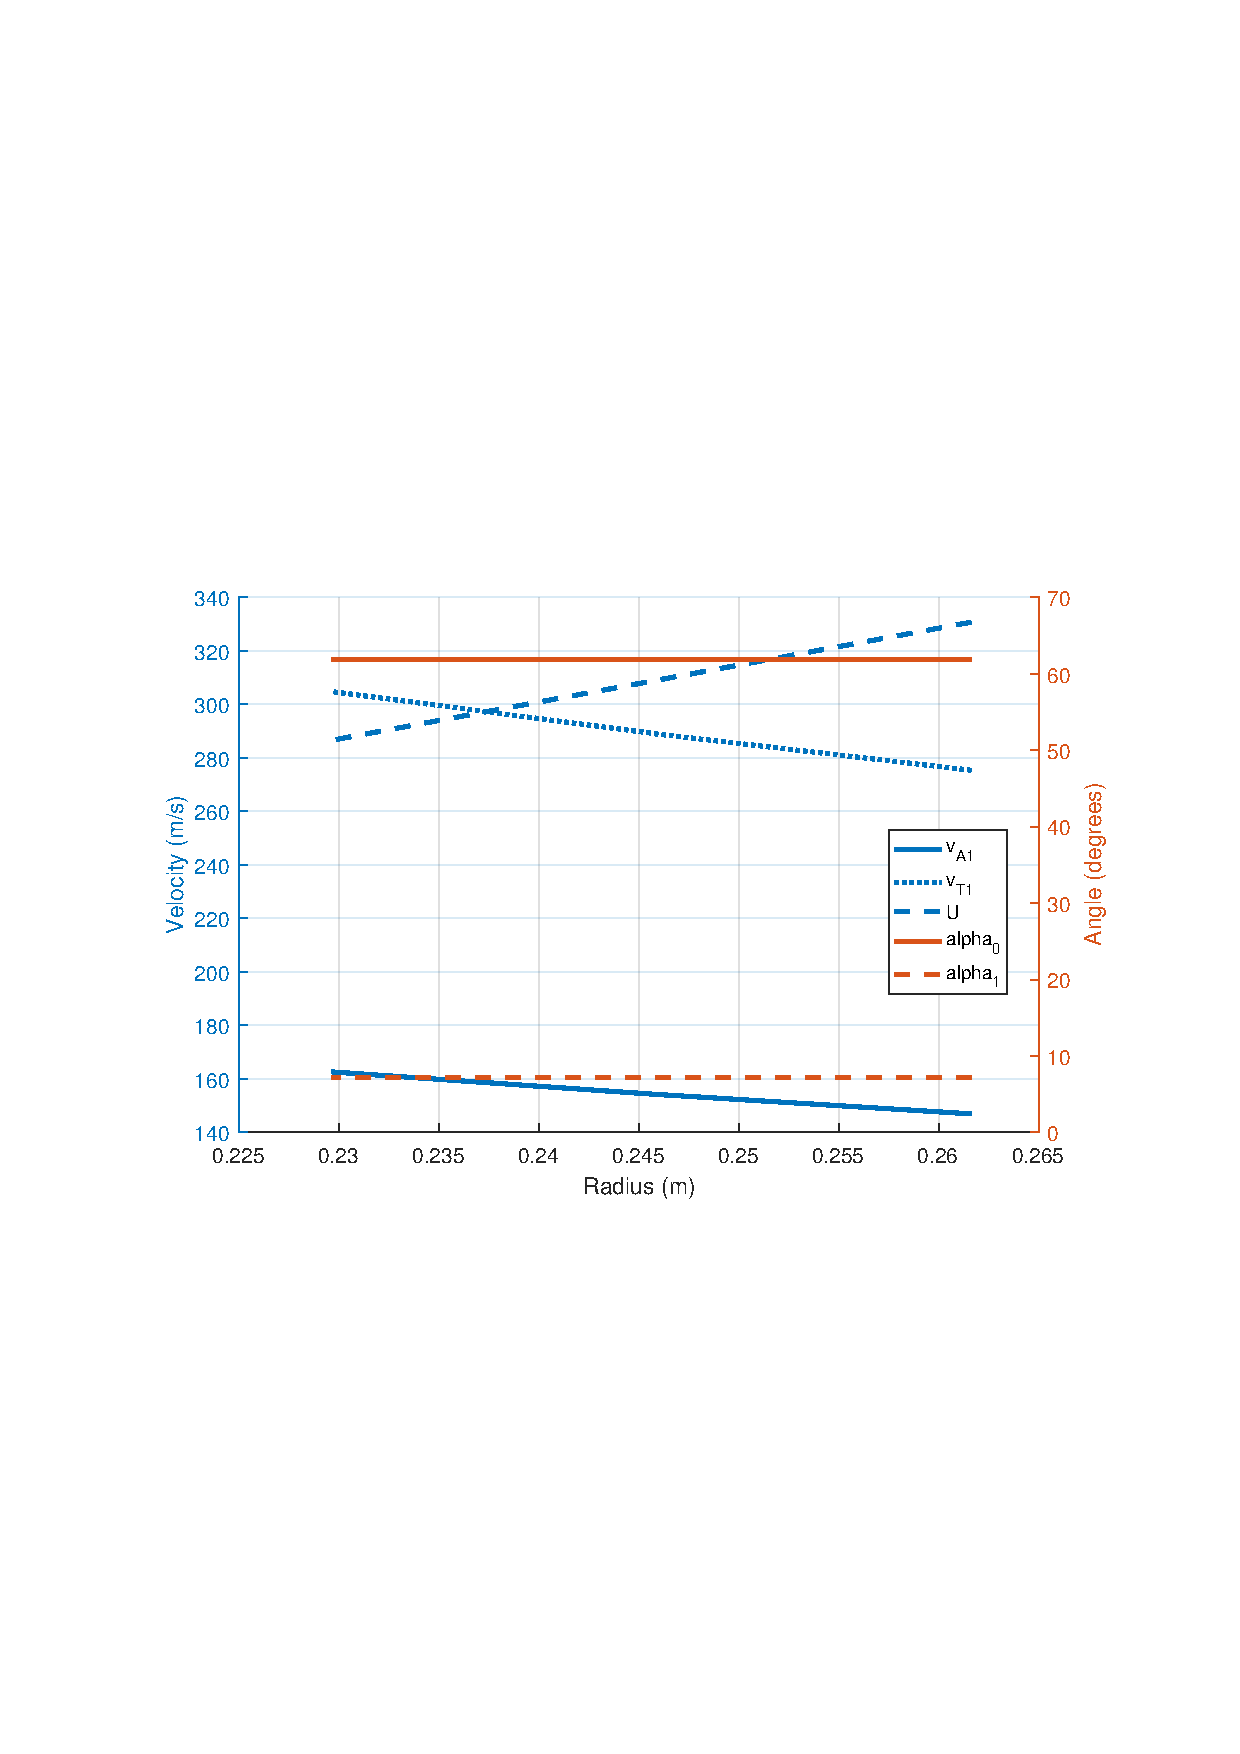
\includegraphics[scale=0.6]{fig/velocity_span_example.pdf}
\end{figure}
\end{frame}

\begin{frame}[t]{The model of the machine - Section solution}
The span velocity is required to compute a better value for the blade height from the mass flow rate.
\begin{equation}
\label{eq:mass_flow_rate_integral}
\dot{m} = \int_{r_\text{hub}}^{r_\text{tip}} \rho(r) \cdot 2 \, \pi \, r \cdot v_A(r) dr
\end{equation}
Equation \ref{eq:mass_flow_rate_integral} cannot be solved analytically to find $b = r_\text{tip} - r_\text{hub}$ since the density depends on the steam table.

The solution in to approximate the integral with a summation for some points along the span.

The number of point an input, but their \highlightgreenC{\textbf{location}} is chosen \highlightgreenC{\textbf{smartly}}.

\myspace
\myspaceneg
The solution is in the form:
\myspaceneg
\begin{equation}
\dot{m} \simeq \sum_i^{\text{N points}} w_i \cdot \rho_i \, v_{A_i} \, \pi \dmid \, \varepsilon \, b 
= b \cdot \left( \pi \dmid \, \varepsilon \cdot \sum_i^{\text{N points}} w_i \cdot \rho(r_i) \, v_{A}(r_i)  \right)
\end{equation}
\end{frame}

\begin{frame}[t]{The model of the machine - Section solution}
The radius at which we compute the solution are chosen according to the following rule:

\begin{equation}
r_i = \frac{\dmid - b}{ 2} +  x_i \cdot b
\end{equation}
Where the first guess of b is taken from the midspan solution.
The coefficients $x_i$ and $w_i$ are taken form the \highlightgreenC{\textbf{Legendre-Gauss quadrature}} technique.
For the case of 4 points for example the coefficients result:
\begin{center}
\begin{tabular}{|c|c|}
\hline 
$x_i$ & $w_i$ \\ 
\hline 
0.9306 & 0.1739 \\ 
\hline 
0.67 & 0.3261 \\ 
\hline 
0.33 & 0.3261 \\ 
\hline 
0.0694 & 0.1739 \\ 
\hline 
\end{tabular} 
\end{center}
\end{frame}

\begin{frame}[t]%{The model of the machine - Gauss points}
%In the following figure is show the sum of the blade height of all the stages for different number of stages.
\myspaceneg
\myspaceneg
\myspaceneg
\myspaceneg
\begin{figure}[hbtp]
\caption{Influence of the choise of the number of Gauss points}
\centering
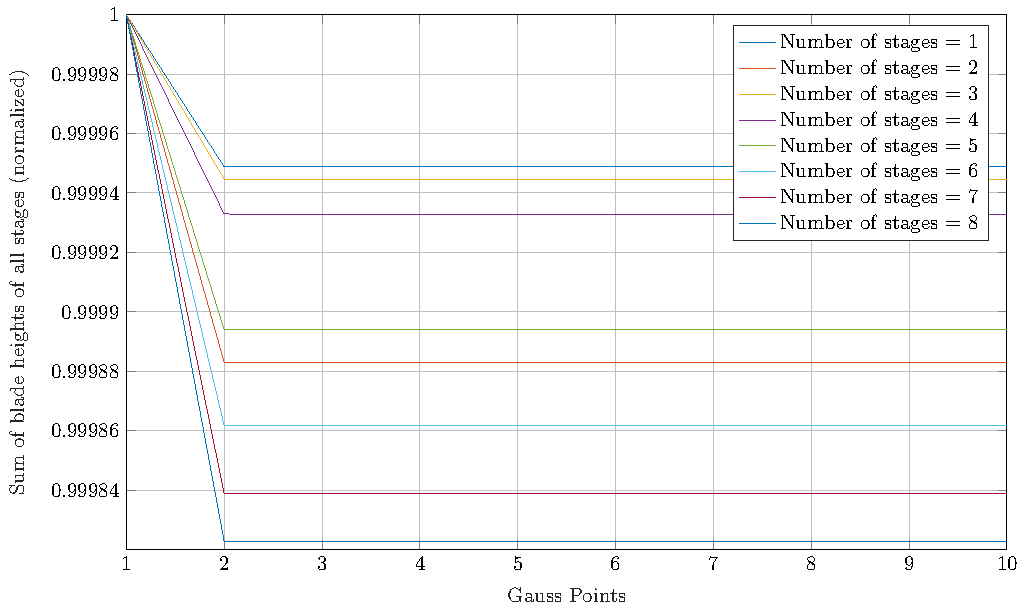
\includegraphics[scale=0.55]{fig/ngauss_example.pdf}
\end{figure}
	
\myspaceneg
\myspaceneg
\myspaceneg
We can notice that the difference is absolutely negligible for a number of Gauss points greater than 2.
For safety region we will use 4 points to be sure not to lose precision and to have a better span evolution
	
\end{frame}


\begin{frame}[t]{The model of the machine - Section solution}
So we start a new iterative process to find the \highlightgreenC{\textbf{blade height}}.

In this process we need the density along the span. 

\begin{center}
$\Rightarrow$ We have to pass from the loss coefficient.
\end{center}

Loss coefficient accounts for 3 contributions:
\begin{itemize}
	\item profile losses $\leftarrow$ local property 
	\item clearance losses  $\leftarrow$ global property 
	\item secondary losses  $\leftarrow$ global property 
\end{itemize} 

\myspace
So along the span we compute the specific \highlightgreenC{profile losses} that depends on the velocity triangle, but we keep the others from the midspan.

%\begin{center}
%\highlightgreenD{\textbf{Doing this we have made the strong assumption that the fluid flows along almost parallel streamlines.}}
%\end{center}
\end{frame}


\begin{frame}[t]
So we have two other iterative loops inside the main one.

\begin{figure}[hbtp]
\centering
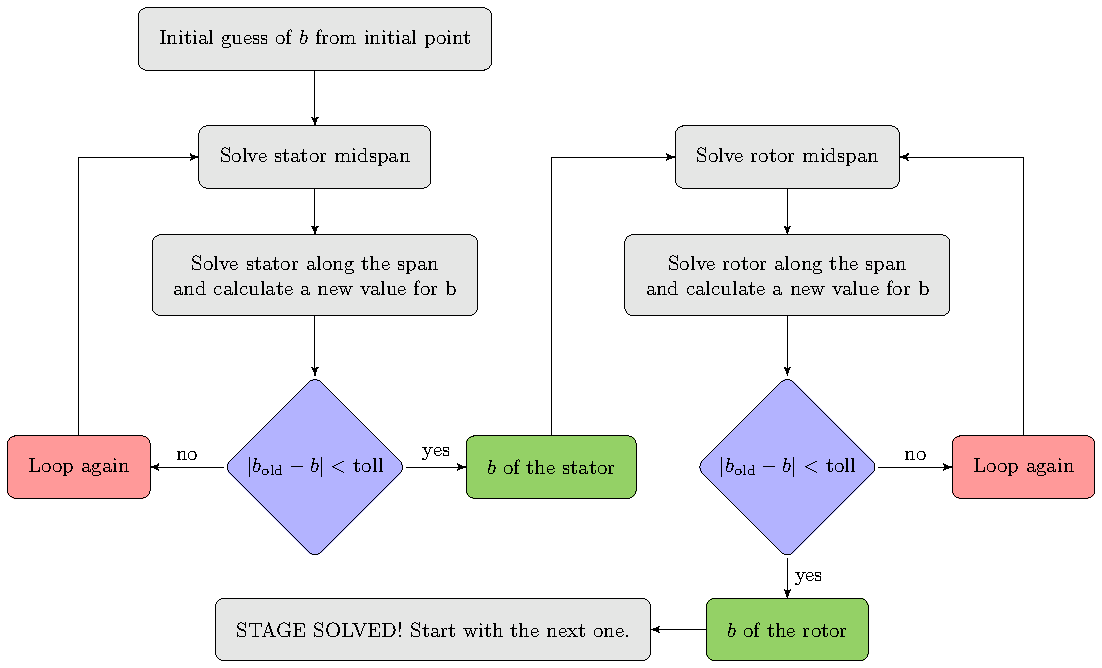
\includegraphics[scale=0.6]{fig/secondaryloop_fig.pdf}
\end{figure}

\end{frame}


\begin{frame}[t]{The model of the machine - The end of the loop}
Repeating the loop sketched in the previous slide for all the stages we completely solve the thermodynamics of all the points of interest.

From all the data we collect we can verify that the total pressure ratio is that desired and we can compute the efficiency of each stage.

\myspace
Finally we can calculate the most important parameter, the \highlightgreenC{\textbf{total to total efficiency}} that we have guess at the beginning.
\begin{equation}
h_{T_\text{end}}^\text{isoentropic} = h(p_T^\text{end}, s_0)
\end{equation}
\begin{equation}
\eta_{\text{TT}} = \frac{h_{T0} - h_T^{\text{end}}}{h_{T0} - h_{T_{\text{end}}}^{\text{isoentropic}}}
\end{equation}
If convergence is not reached the main loop start again.
\end{frame}

\begin{frame}[t]{The model of the machine - Effective work}
Applying constant angle methodology the work is not constant along the span, so per each stage we can compute the effective work and compare to the real one.

\myspace
If the difference is significant we have to redesign the velocity triangles to guarantee that the expansion work is that desired.
We can take a mean along the span weighting on the mass flow or on the Gauss weight.

\begin{equation}
l  \simeq \frac{\sum_i^{\text{N points}} w_i \cdot u_i \cdot (w_{1T_i} - w_{2T_i}) \cdot \pi \, \dmid \, b \cdot \rho_i \, v_{Ai}}{\dot{m}} 
\end{equation}
%l  \simeq \sum_i^{\text{N points}} w_i \cdot u(r_i) \cdot (v_{1T}(r_i) - v_{2T}(r_i) ) = \sum_i^{\text{N points}} w_i \cdot u_i \cdot (w_{1T_i} - w_{2T_i} )
The difference due to small blade height in high pressure part of the turbine is negligible.
\end{frame}


\begin{frame}
\begin{figure}[hbtp]
\centering
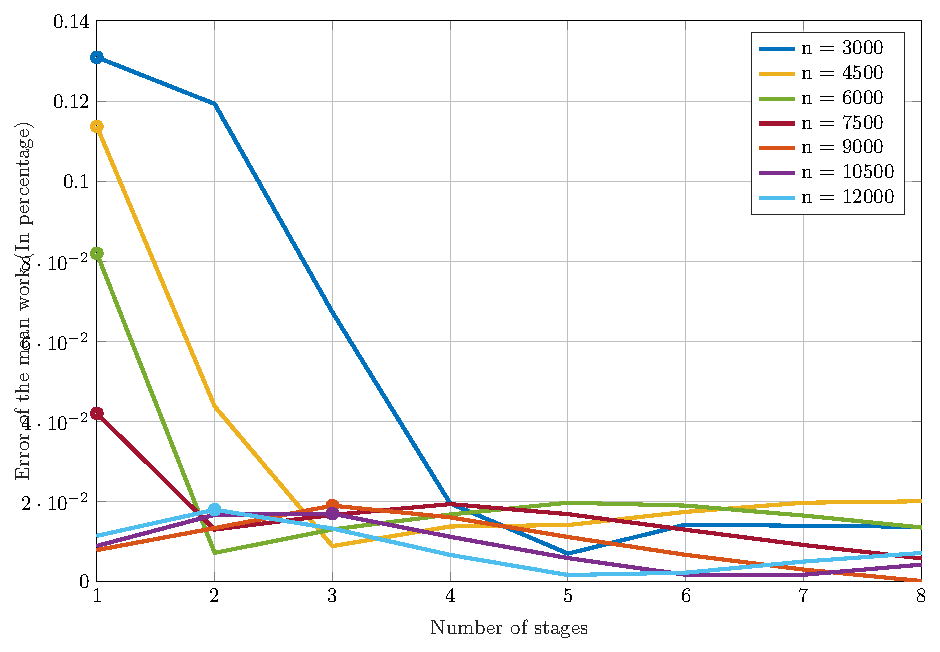
\includegraphics[scale=0.65]{fig/work_error_perc_example.pdf}
\end{figure}
\end{frame}


\begin{frame}
\begin{center}
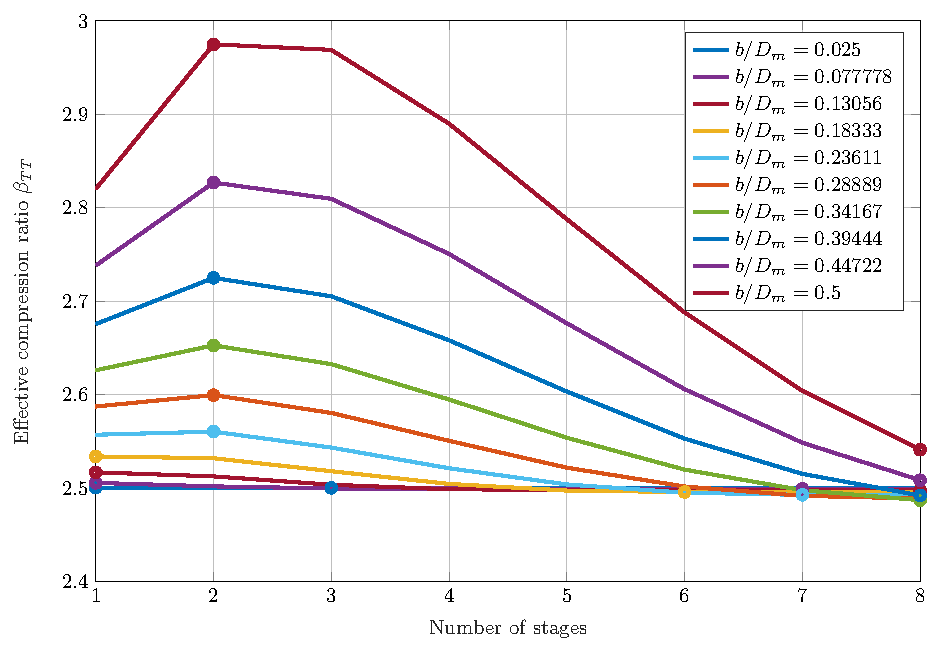
\includegraphics[scale=0.65]{fig/betareal_bsuD_example.pdf} 
\end{center}
\myspaceneg
\myspaceneg
\begin{center}
In mid or low pressure turbine the assumption could be not true.
\end{center}
\end{frame}


\begin{frame}[t]{The model of the machine - The losses}
Up to now we have simply spoken of rotor and stator losses in a generic way without explaining how to evaluate them.
The losses are divided in 3 groups:
\begin{itemize}
	\item Profile losses;
	\item Secondary losses;
	\item Clearance losses.
\end{itemize}
As previously stated the last two are evaluated by the model as mean losses along the section.

\begin{center}
The calculation of profile losses is performed according to the \highlightgreenC{\textbf{Ainley-Mathieson}} correlation. 
\end{center}

\begin{center}
The calculation of others instead is performed according to the \highlightgreenC{\textbf{Dunham-Came}} correlation.
\end{center}
\end{frame}


\begin{frame}[t]{The model of the machine - Profile losses}
Profile losses are calculated in a general case with a linear interpolation between:
\begin{itemize}
	\item axial inlet with $\chi = 0.5$ ($\alpha_0 = 0$)
	\item symmetrical blades ($\alpha_0 = - \alpha_1$)
\end{itemize}
\vspace{-0.5cm}
\begin{figure}%
    \centering
    \subfloat{{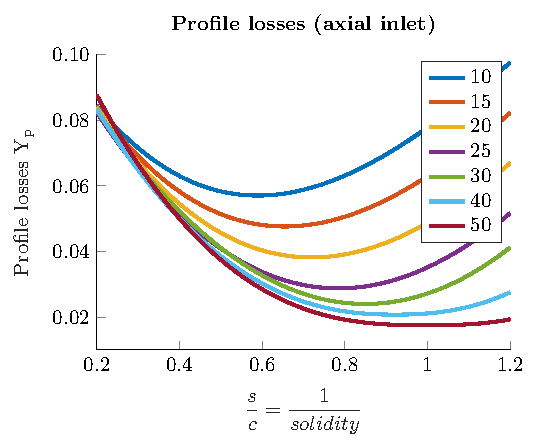
\includegraphics[height=4.5cm]{fig/profile_losses1.pdf} }}%
    \subfloat{{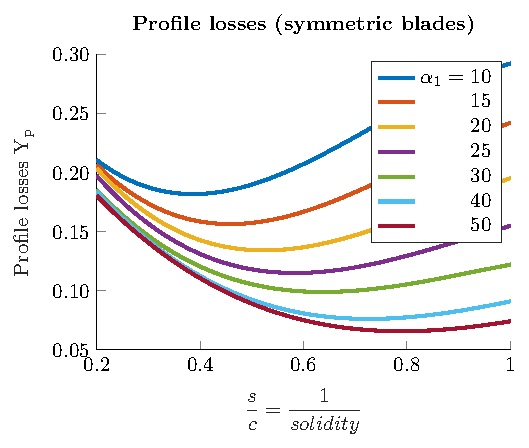
\includegraphics[height=4.5cm]{fig/profile_losses2.pdf} }}%
    \label{fig:profile_losses}%
\end{figure}
\end{frame}



\begin{frame}[t]{The model of the machine - Profile losses}
We compute the total pressure losses in both cases and than we apply the following interpolation:

\myspaceneg
\myspaceneg
\begin{equation}
Y_{p_\text{reference}} = Y_A + m_\alpha^2 \, ( Y_B - Y_A) 
\end{equation}
Where $m_\alpha = -\alpha_0 / \alpha_1$.
Then we apply further corrections:
\begin{center}
\begin{itemize}
	\item \begin{center} Max thickness: $Y_p = Y_{p_\text{ref}} \cdot \left( \dfrac{t_\text{max} / c}{t_\text{max} / c \vert_\text{ref}} \right) ^ {m_\alpha}$ \end{center}
	\item \begin{center} Reynolds: $Y_p = Y_{p_\text{ref}} \cdot \left( \dfrac{\text{Re}_\text{ref}}{\text{Re}} \right)^{\!0.2}$ \end{center}
	\item \begin{center} Trailing edge: $Y_p = Y_{p_\text{ref}} \cdot \left( 1 + 7\, \left(\dfrac{t}{s} - \left. \dfrac{t}{s} \right\vert _\text{ref} \right) \right)$ \end{center}
\end{itemize}
\end{center}
Where the Reynolds number is that referred to the chord and values:
\begin{equation}
\text{Re} = \dfrac{\rho_0\,\overline{v}\,c}{\mu_0}
\end{equation}
\end{frame}


\begin{frame}[t]{The model of the machine - The solidity}
The main parameter that influences profile losses is the \highlightgreenC{\textbf{solidity}}
Even if it can be chosen arbitrarily it must be subjected to the number of blades that is instead an \emph{integer}.
So the solidity is computed passing through a rounding operation.

\myspaceneg
\myspaceneg
\begin{equation}
\text{N}_\text{blades} = \text{round}\left( \dfrac{\pi\,\dmid}{c} \cdot \sigma  \right) 
\end{equation}
And then we recalculate the solidity.
\begin{equation}
\label{eq:solidity_from_nblades}
\sigma = \dfrac{c}{s} = \dfrac{c}{\pi\,\dmid} \cdot \text{N}_\text{blades}
\end{equation}
Than when we calculate profile losses along the span we keep that number of blades and recalculate 
the solidity in the same way as equation \ref{eq:solidity_from_nblades}
with the new value of the diameter.
\end{frame}



\begin{frame}[t]{The model of the machine - Secondary losses}
Secondary losses are accounted as follow:
\begin{equation}
Y_\text{secondary} = 0.0334 \, \dfrac{\cos(\alpha_1)}{\cos(\alpha_0)} \cdot H
\end{equation}
\begin{equation}
\label{eq:coef_losses}
H = 4\, \dfrac{c}{b} \left( \tan\alpha_0 - \tan\alpha_1 \right) ^2 \cdot \dfrac{\cos^2(\alpha_1)}{\cos(\alpha_m)}
\end{equation}
\begin{equation}
\tan\alpha_m = \dfrac{\tan\alpha_0 + \tan\alpha_1}{2}
\end{equation}
Every loss equation in the way it is written holds for a stator, for a rotor instead we must replace
\begin{itemize}
	\item \begin{center} $\alpha_0 \Leftrightarrow \beta_1$ \end{center}
	\item \begin{center} $\alpha_1 \Leftrightarrow \beta_2$ \end{center}
\end{itemize}
\end{frame}


\begin{frame}[t]{The model of the machine - Clearance losses}
Secondary losses are accounted as follow:
\begin{equation}
Y_\text{clearance} = B \, \left( \dfrac{k}{c} \right)^{0.78} \cdot H
\end{equation}
Where H has been previously defined in equation \ref{eq:coef_losses}
The term $k$ is the clearance normalized respect to the number of seals.
\begin{equation}
k = \left( \dfrac{\text{clearance}}{\text{seals number}} \right)^{0.42}
\end{equation}

The coefficient $B$ distinguish between the stator and the rotor and for the type of casing.

\myspaceneg
\myspaceneg
\myspaceneg
\[
B = 
   \begin{dcases}
     0 & \text{stator} \\
     \highlightgreenC{\textbf{0.37}} & \highlightgreenC{\text{\textbf{shrouded rotor}}} \\
     0.47 & \text{unshrouded rotor}
   \end{dcases}
\]
\end{frame}


\begin{frame}[t]{The choice of parameters - Reference condition}

\myspaceneg
When testing many configurations, we keep for parameters which are note analysed the following values:
\begin{itemize}
	\item solidity $\sigma = 1.225$
	\item number of stages $n_\text{stages} = 4$
	\item rotational speed $n = 6000\,\text{rpm}$
	\item reaction degree at midspan $\chi = 0.5$
	\item flow coefficient $\phi = 0.5$
	\item partial admission $\varepsilon = 1$
	\item blade height over mean diameter $b / \dmid = 0.05$
	\item blade height over chord $b / c = 0.5$
	\item seals number $= 2$
	\item clearance $ = \round[round-precision=4]{0.02 * 0.03} \m$
\end{itemize}

\end{frame}

\begin{frame}[c]{The choice of parameters - The solidity}
\begin{figure}%
    \centering
    \subfloat{{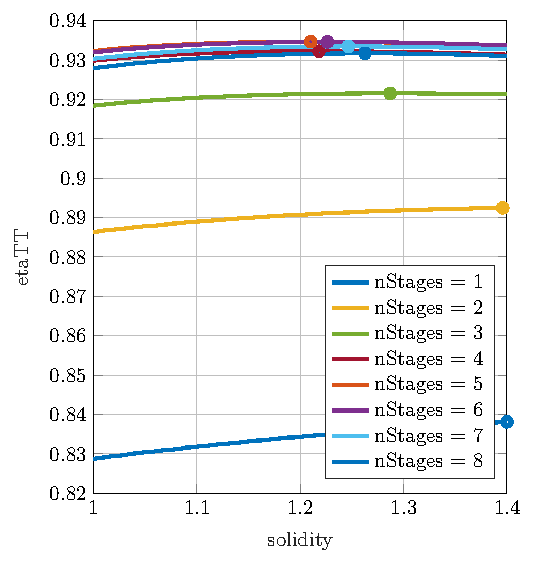
\includegraphics[height=6cm]{fig/solidity_nstages.pdf} }}%
    \subfloat{{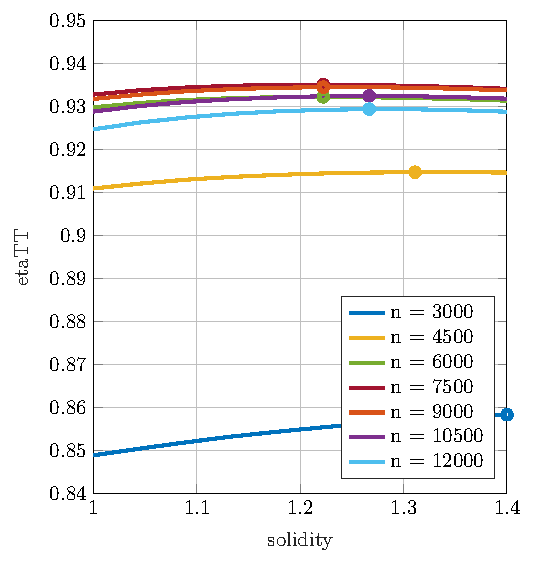
\includegraphics[height=6cm]{fig/solidity_rpm.pdf} }}%
\end{figure}
\end{frame}

\begin{frame}[c]{The choice of parameters - The solidity}
\begin{figure}[c]%
    \centering
    \subfloat{{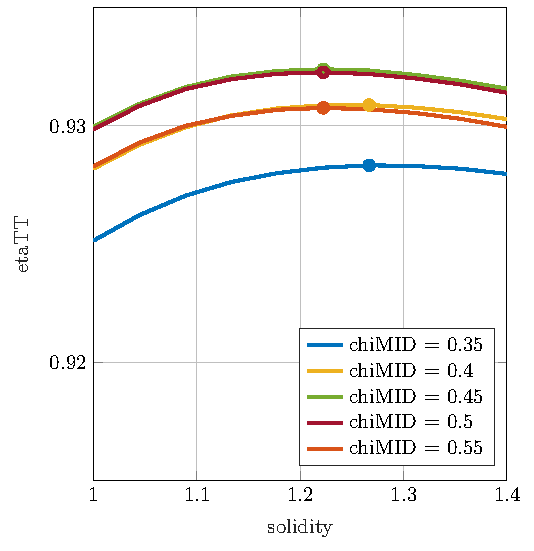
\includegraphics[height=6cm]{fig/solidity_chimid.pdf} }}%
    \subfloat{{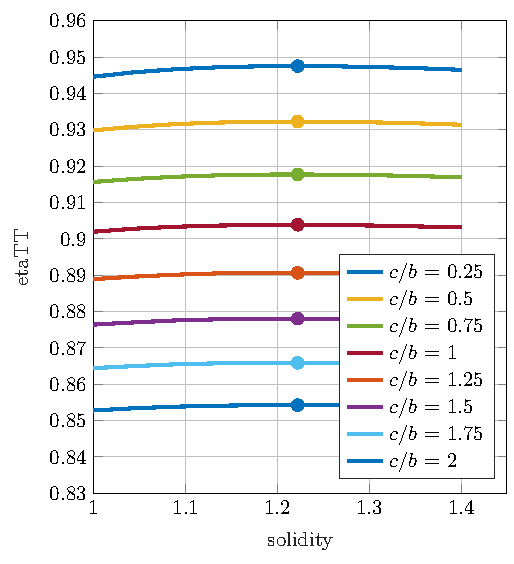
\includegraphics[height=6cm]{fig/solidity_chordsub.pdf} }}%
\end{figure}
\end{frame}



%\begin{figure}[hbtp]
%\centering
%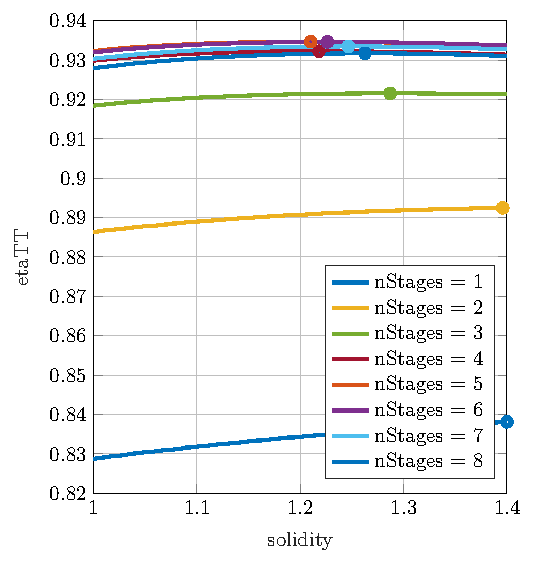
\includegraphics[scale=0.85]{fig/solidity_nstages.pdf}
%\end{figure}
%\end{frame}
%
%\begin{frame}[t]{The choice of parameters - The solidity}
%\begin{figure}[hbtp]
%\centering
%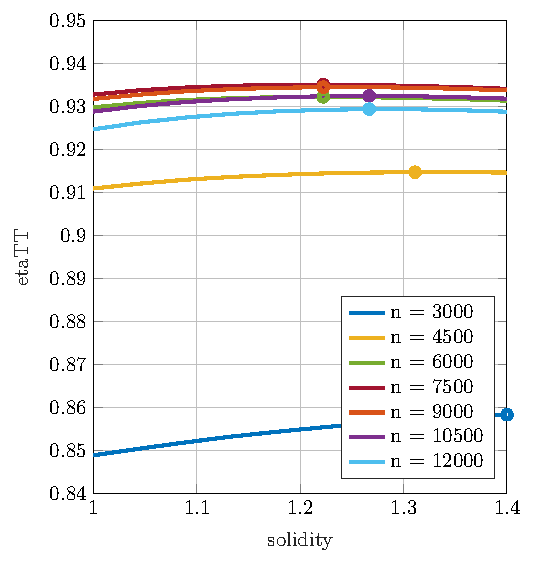
\includegraphics[scale=0.85]{fig/solidity_rpm.pdf}
%\end{figure}
%\end{frame}
%
%\begin{frame}[t]{The choice of parameters - The solidity}
%\begin{figure}[hbtp]
%\centering
%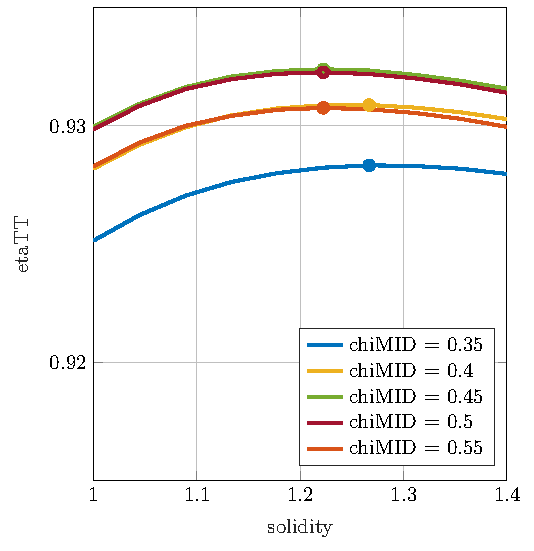
\includegraphics[scale=0.85]{fig/solidity_chimid.pdf}
%\end{figure}
%\end{frame}
%
%\begin{frame}[t]{The choice of parameters - The solidity}
%\begin{figure}[hbtp]
%\centering
%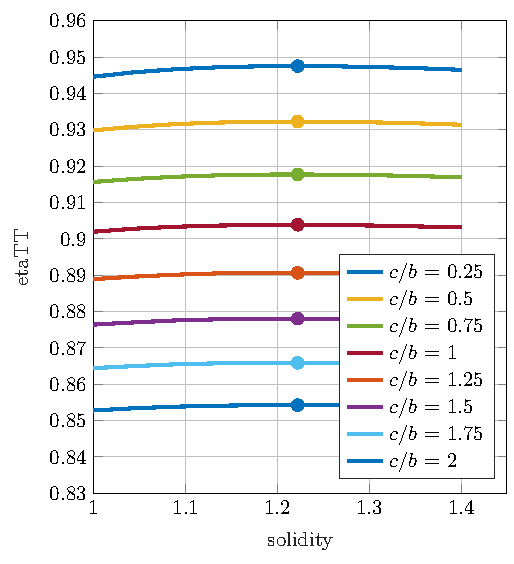
\includegraphics[scale=0.85]{fig/solidity_chordsub.pdf}
%\end{figure}
%\end{frame}


\begin{frame}[t]{The choice of parameters - The solidity}
Even if the solidity is a key parameter for the performances of the machine, 
keeping into a reasonable range suggested by the theory, it not influences too much the efficiency.

\myspace
\myspaceneg
From the analysis of the previous graphs seems reasonable to pick a value of the solidity of 1.225;
\begin{center}
\large{\highlightgreenC{Solidity $\sigma = 1.225$}}
\end{center}

\myspaceneg
\myspaceneg
\myspaceneg
\begin{figure}[hbtp]
\centering
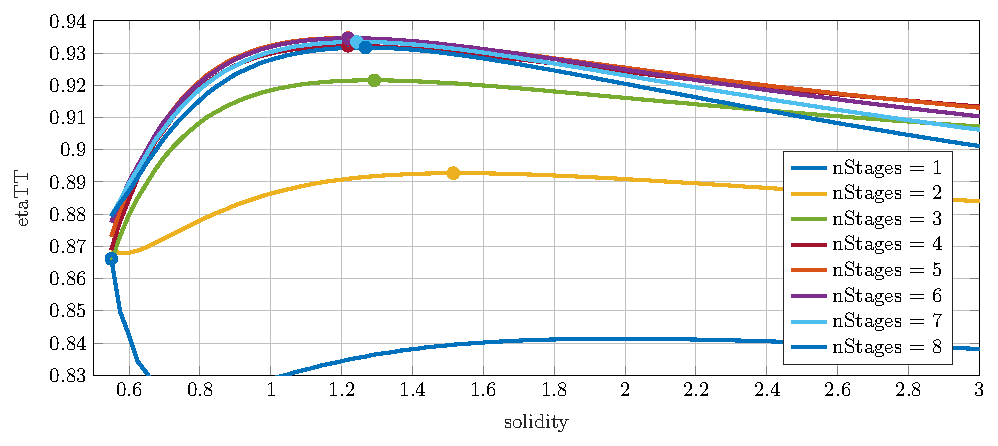
\includegraphics[scale=0.47]{fig/solidity_wrong.pdf}
\end{figure}
\end{frame}


\begin{frame}[t]{The choice of parameters - The solidity}

\myspaceneg
\myspaceneg
\myspaceneg
\begin{wrapfigure}{R}{200pt}
\centering
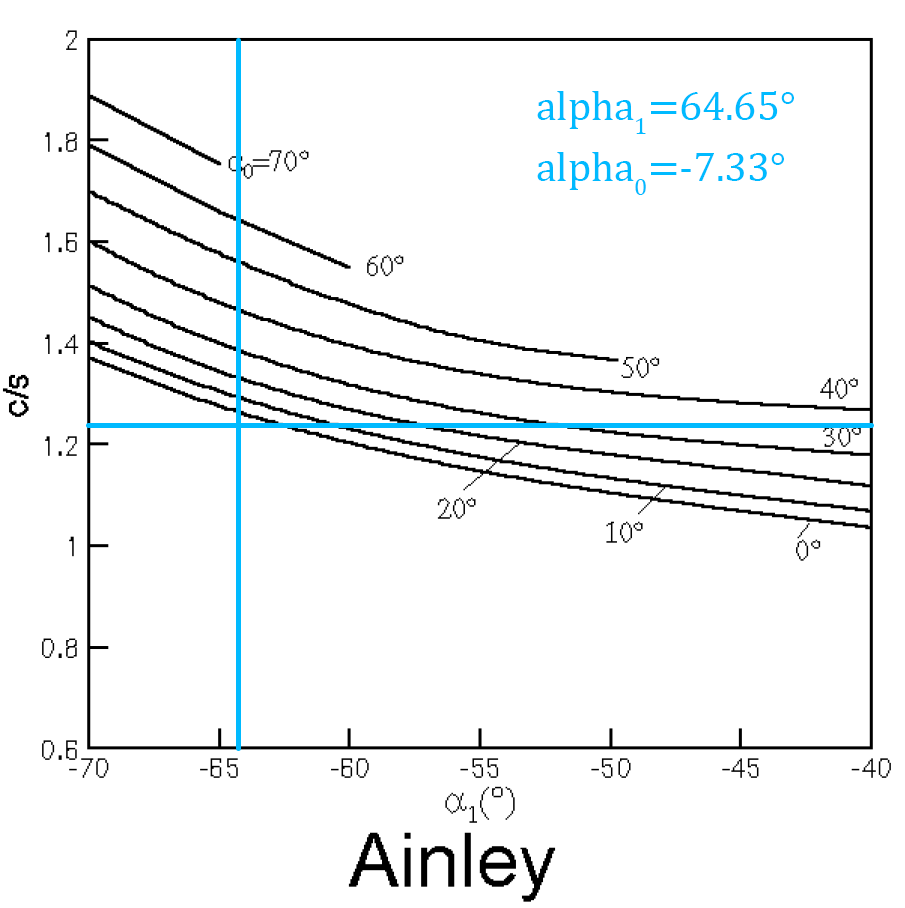
\includegraphics[width=6cm]{fig/ainley_loading.png}
\caption{Ainley criterion}
\label{fig:ainley_loading}
\end{wrapfigure}

\leavevmode
\newline
\newline
\newline
Comparison of the solidity with \highlightgreenC{\textbf{loading criterion of Ainley}}. 
%\begin{figure}[hbtp]
%\centering
%\label{fig:ainley_loading}
%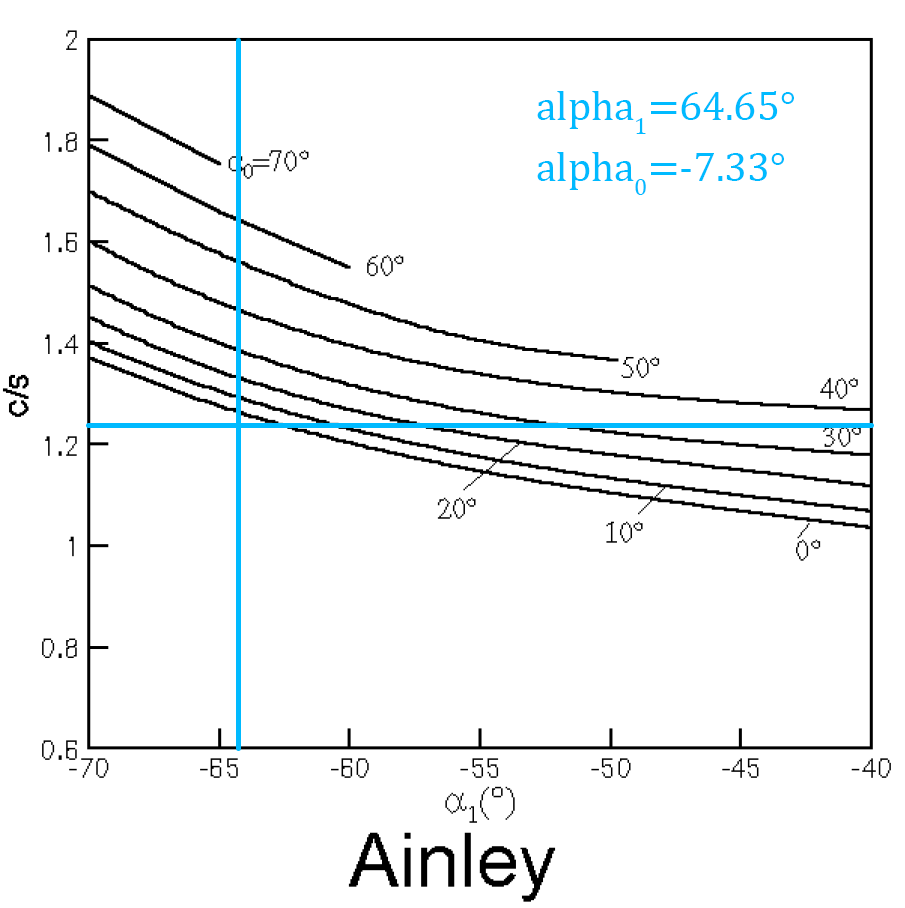
\includegraphics[scale=0.8]{fig/ainley_loading.png}
%\end{figure}

\myspace
As we see in figure \ref{fig:ainley_loading} the value that we take is very similar to that predicted by the Ainley loading criterion.
\end{frame}


\begin{frame}[t]{The choice of parameters - The reaction degree}
The reaction degree at midspan is also a relevant parameter. 
\begin{center}
If too low, the stator is too loaded.
\end{center}

\begin{center}
If too high the load is mainly on the rotor.
\end{center}

From the theory we know that a mean between this two extreme condition let to have a good result.

So we check what is the reaction degree that gives the better performances around $\chi = 0.5$.
\end{frame}

\begin{frame}[t]{The choice of parameters - The reaction degree}

\begin{center}
A good value for $\chi$ seams to be 0.47, just a bit less than 0.5.
\end{center}

\vspace{-1cm}
\begin{figure}
    \centering
    \subfloat{{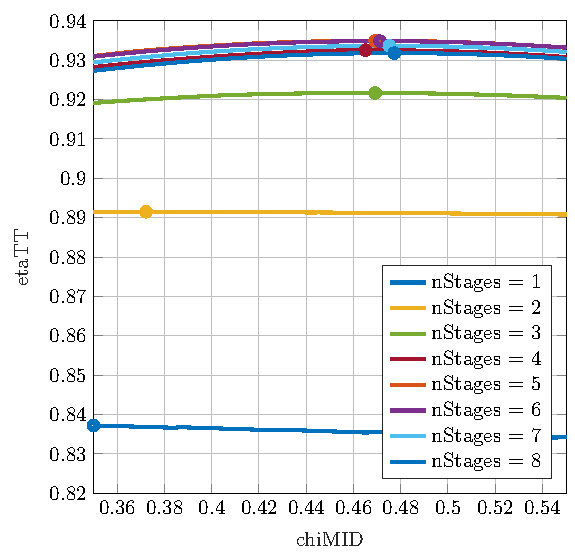
\includegraphics[height=5.5cm]{fig/chi_nstages.pdf} }}%
    \subfloat{{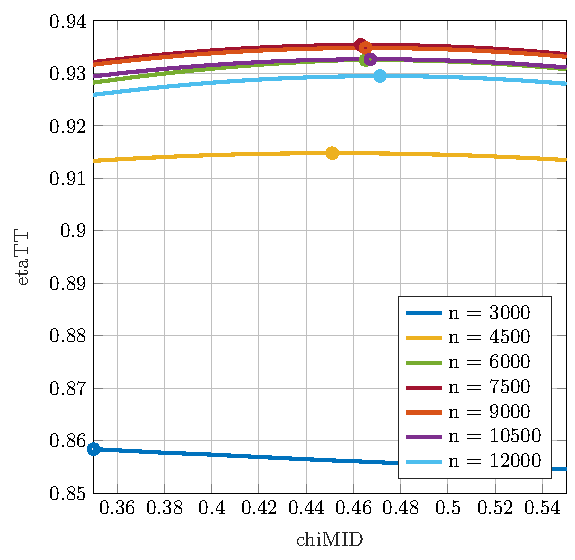
\includegraphics[height=5.5cm]{fig/chi_rpm.pdf} }}%
\end{figure}


%\begin{figure}[hbtp]
%\centering
%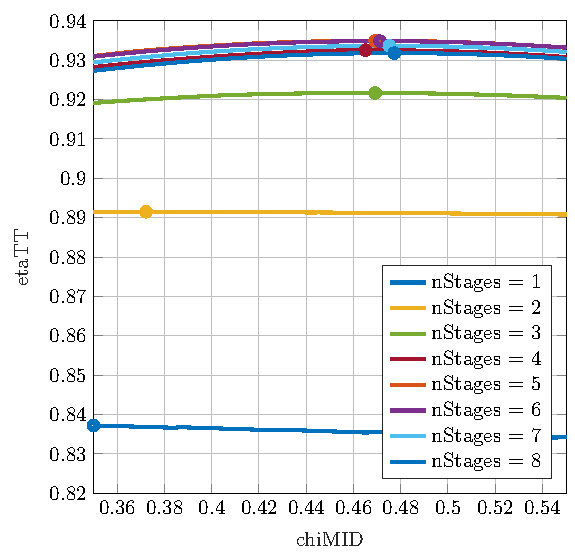
\includegraphics[scale=0.85]{fig/chi_nstages.pdf}
%\end{figure}
%\end{frame}
%
%\begin{frame}[t]{The choice of parameters - The reaction degree}
%\myspaceneg
%\myspaceneg
%\begin{figure}[hbtp]
%\centering
%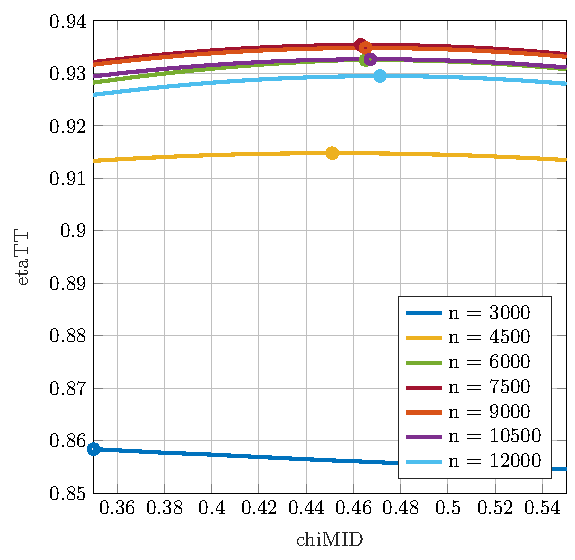
\includegraphics[scale=0.85]{fig/chi_rpm.pdf}
%\end{figure}

\end{frame}


\begin{frame}[t]{The choice of parameters - The reaction degree}
It is also interesting to analyse the graphs in a reverse way, to start to check the best value for the \emph{number of stages} and the \emph{rotational speed}.

\vspace{-0.5cm}
\begin{figure}%
    \centering
    \subfloat{{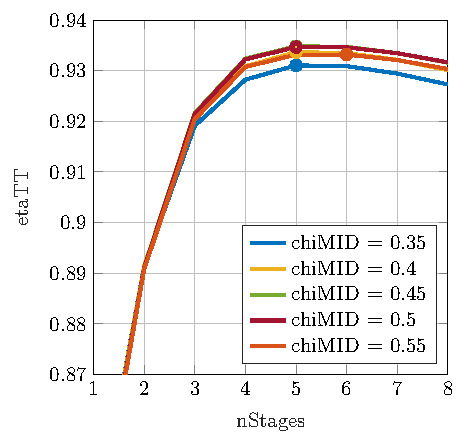
\includegraphics[height=5.5cm]{fig/chi_nstages_reverse.pdf} }}%
    \subfloat{{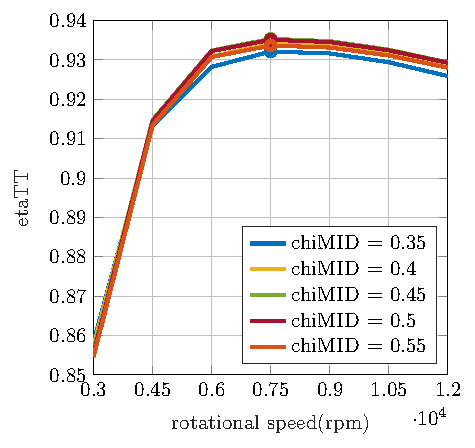
\includegraphics[height=5.5cm]{fig/chi_rpm_reverse.pdf} }}%
\end{figure}
\end{frame}



\begin{frame}[t]{The choice of parameters - Clearance and seals}
From 1 to 2 seals we have a good increase in efficiency that is decreases so we take 2 seals per rotor.

\vspace{-0.5cm}
\begin{figure}%
    \centering
    \subfloat{{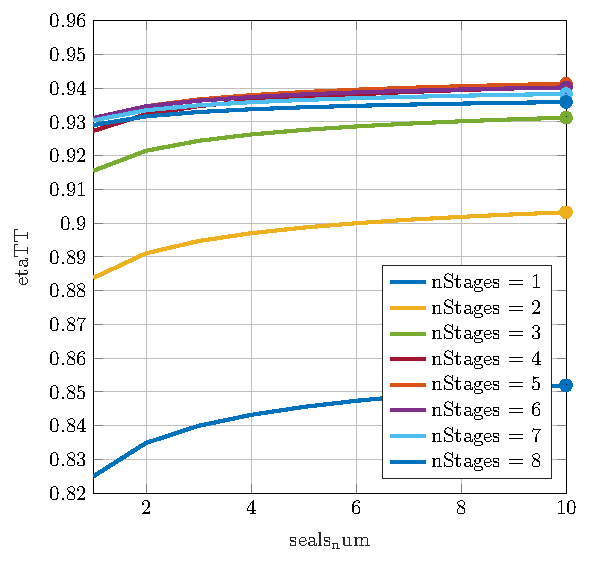
\includegraphics[height=5.5cm]{fig/seals_nstages.pdf} }}%
    \subfloat{{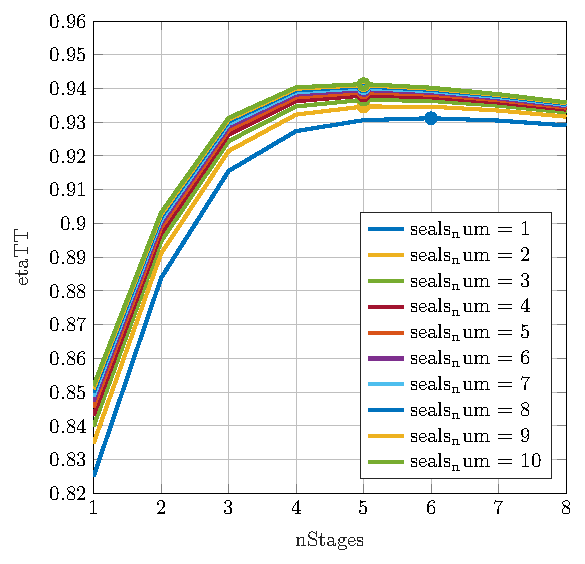
\includegraphics[height=5.5cm]{fig/seals_nstages_reverse.pdf} }}%
\end{figure}
\end{frame}

\begin{frame}[t]{The choice of parameters - Clearance and seals}
Decreasing the clearance the efficiency increases.

We take as clearance $k \approx 0.02 \cdot b \approx 0.5\, \text{mm}$.

\vspace{-0.5cm}
\begin{figure}%
    \centering
    \subfloat{{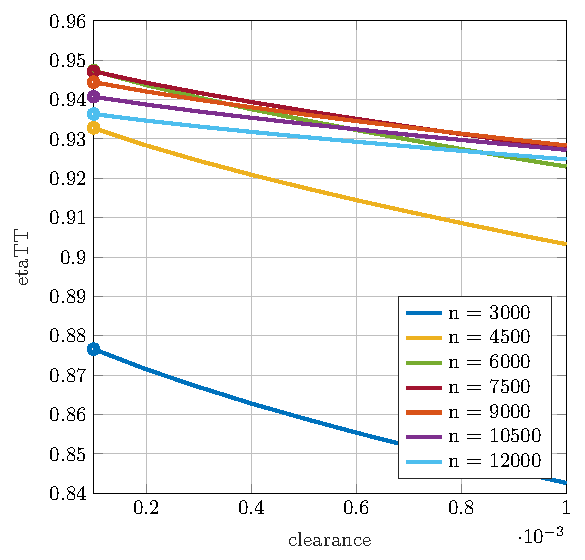
\includegraphics[height=5.5cm]{fig/clearance_rpm.pdf} }}%
    \subfloat{{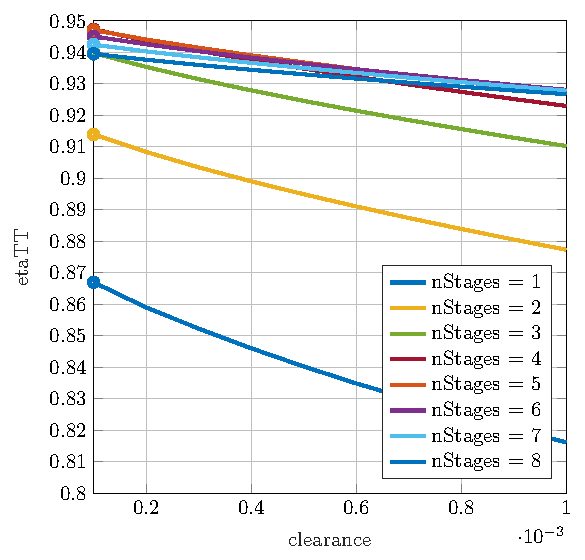
\includegraphics[height=5.5cm]{fig/clearance_nstages.pdf} }}%
\end{figure}
\end{frame}


\begin{frame}[t]{The choice of parameters - Stages and speed}

\myspaceneg
\myspaceneg
For any number of stages exists a proper value of the rotational speed that let to reach almost the same efficiency.
Critical decision:

$\Rightarrow$ at $3000 \text{rpm}$, good efficiency for over 10 stages.

$\Rightarrow$ for 2 stages, good efficiency for $n$ above $10000 \text{ rpm}$.

\vspace{-0.8cm}
\begin{figure}%
    \centering
    \subfloat{{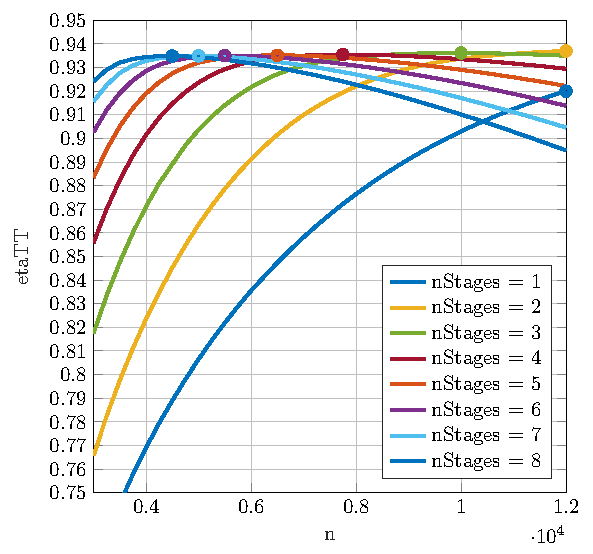
\includegraphics[height=5.25cm]{fig/n_nstages.pdf} }}%
    \subfloat{{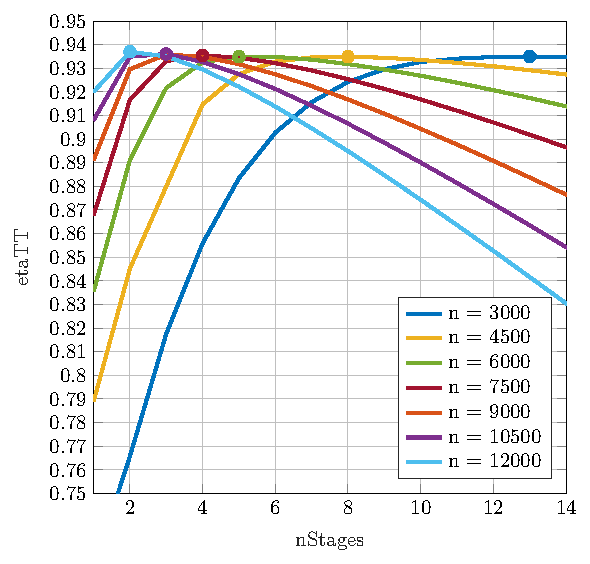
\includegraphics[height=5.25cm]{fig/n_nstages_reverse.pdf} }}%
\end{figure}
\end{frame}



\begin{frame}[t]{The choice of parameters - Stages and speed and phi}

\myspaceneg
\myspaceneg
\begin{center}
For $\phi = 0.4469$ we have the optimal efficiency at:

\textbf{$\Rightarrow$ \highlightgreenC{4 stages};}

\textbf{$\Rightarrow$ \highlightgreenC{$\mathbf{n}$ = 6000 rpm};}
\end{center}

\vspace{-0.4cm}
\begin{figure}%
    \centering
    \subfloat{{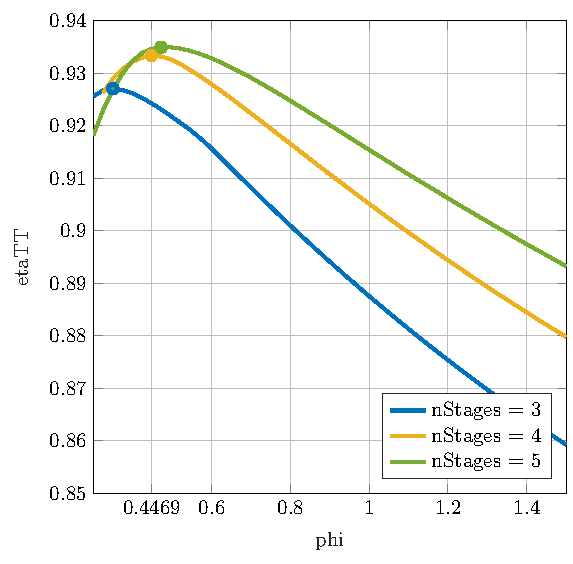
\includegraphics[height=5.25cm]{fig/phi_nstages_small.pdf} }}%
    \subfloat{{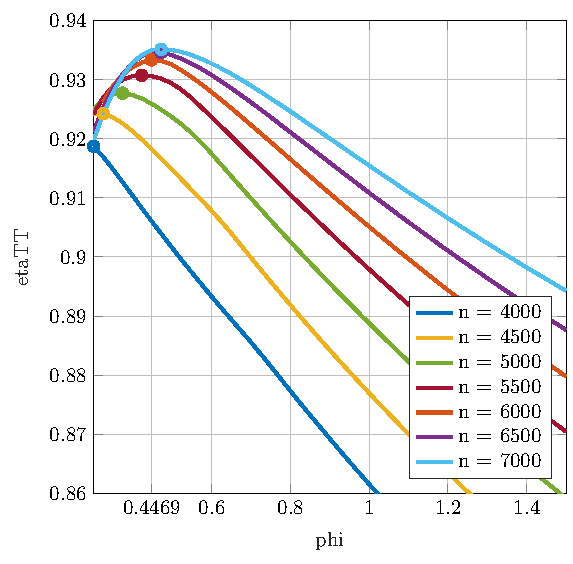
\includegraphics[height=5.25cm]{fig/phi_rpm_small.pdf} }}%
\end{figure}
\end{frame}





\begin{frame}[t]{The design of the blades}
The blades are designed according two different rules:
\begin{itemize}
	\item NACA 4-digits for the mean line;
	\item $A_3K_7$ for the thickness.
\end{itemize}
\begin{figure}[hbtp]
\centering
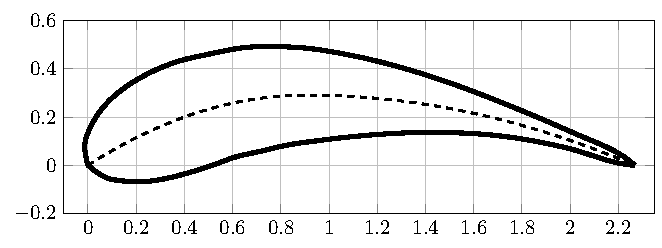
\includegraphics[scale=0.85]{fig/rotor_blade.pdf}
\caption{Example of a rotor blade with max thickness over chord of 0.2}
\end{figure}
\end{frame}


\begin{frame}[t]{The design of the blades - The mean line}
Calling $m$ the maximum of the mean line and $p$ the position between 0 and 1 at which the maximum is present,
the equation of the mean line are represented by a \highlightgreenC{parabola}.

\[
B = 
   \begin{dcases}
     \dfrac{m}{p^2}\,(2\,p\,x - x^2) & \text{for } x < p \\
     \dfrac{m}{(1-p)^2}\,(1 - 2\, p + 2\,p\,x - x^2) & \text{for } x \geq p
   \end{dcases}
\]
The advantage of this approach is that we can easily calculate everything we want of the mean line like the \highlightgreenD{slope} or the \highlightgreenD{osculating circle radius}.

\begin{center}
It is reasonable to take $p = 0.4$.
\end{center}
\end{frame}


\begin{frame}[t]{The design of the blades - The mean line}
We miss the parameter m.

We can obtain it from the camber angle required and from p.

\begin{equation}
\tan\theta = \tan(\alpha_0 + \alpha_1) = \dfrac{\tan\alpha_0 + \tan\alpha_1}{1 - \tan\alpha_0 \, \tan\alpha_1}
\end{equation}

Where $\tan\alpha_0 = \frac{2\,m}{p}$ and $\tan\alpha_1 = \frac{2\,m}{1-p}$.

\myspace
Finally $m$ is the solution of the following equation.

\begin{equation}
4 \, \tan(\theta) \, m^2 + 2 \, m + p\,(p-1) \cdot \tan\theta = 0
\end{equation}

\end{frame}



\begin{frame}[t]{The design of the blades - The thickness}

Since the points are quite rough we apply a \highlightgreenC{spline interpolation} to get a smoother profile.

To find the top and bottom points of the blade we project the thickness \highlightgreenD{perpendicular to the mean line}

\myspaceneg
\myspaceneg
%\[
   \begin{eqnarray}
     x_{\text{up}} = x - t \cdot \sin(\atan(y_c^{\prime})) & \quad x_{\text{down}} = x + t \cdot \sin(\atan(y_c^{\prime})) \\
     y_{\text{up}} = x + t \cdot \sin(\atan(y_c^{\prime})) & \quad y_{\text{down}} = x - t \cdot \cos(\atan(y_c^{\prime}))
   \end{eqnarray}
%\]

\begin{table}[]
\resizebox{\columnwidth}{!}{%
\centering
\begin{tabular}{@{}lcccccccccccc@{}}
\toprule
$x / c (\%)$ & 0     & 1.25  & 2.5   & 5     & 10    & 15    & 20    & 25    & 30    & 35    & 40    & 45    \\ 
$t/c$       & 0     & 3.469 & 4.972 & 6.916 & 9.007 & 9.827 & 10    & 9.699 & 9.613 & 9.106 & 8.594 & 7.913 \\ \midrule
$x / c (\%)$ & 50    & 55    & 60    & 65    & 70    & 75    & 80    & 85    & 90    & 95    & 100   &       \\
$t/c$       & 7.152 & 6.339 & 5.5   & 4.661 & 3.846 & 3.067 & 2.406 & 1.83  & 1.367 & 1.101 & 0     &       \\ \bottomrule
\end{tabular}
}
\caption{Thickness along the mean line.}
\end{table}
\end{frame}



\begin{frame}[t]{The design of the blades - The deviation}
Even if the blades drive the flow, at the trailing edge we have just one side that keep it in the desired direction.

\begin{center}
$\Rightarrow$ The flow deviates.
\end{center}

Theroretical 1D approach can provide the result, but the semi-experimental correlations are more reliable.

Ainley and Mathieson provide a correlation for the deviation given:
\begin{itemize}
\item the geometrical angle;
\item the curvature of the suction side $e$\footnote{\raggedleft We approximate it by computing the radius of the circumference passing through the last 3 points of the mean line.};
\item the mach number if greater than 0.5.
\end{itemize}
\end{frame}



\begin{frame}[t]{The design of the blades - The deviation}
We know how to calculate the real flow angle from the geometrical angle but we are interested in the \emph{opposite process}.

We need a specific flow angle that provides the work required by the compression.
\begin{center}
$\Rightarrow$ We want to know the \highlightgreenC{geometric angle} of the blade.
\end{center}
\begin{equation}
\label{eq:alpha_flow_from_geometrical}
\alpha_\text{flow} = f(\alpha_\text{geom}) - 4 \frac{s}{e(\alpha_\text{geom})}
\end{equation}
In the case $M$ is greater than 0.5 we must apply a further correction.
We solve equation \ref{eq:alpha_flow_from_geometrical} by applying the secants method.

\begin{center}
From that solution $\Rightarrow$ design the blade that provides the required work also accounting for the deviation angle.
\end{center}
\end{frame}


\begin{frame}[t]{The results - Losses}
\begin{center}
Losses of the four stages for the stators and the rotors.
\end{center}
\vspace{-0.0cm}
\begin{figure}%
    \centering
    \subfloat{{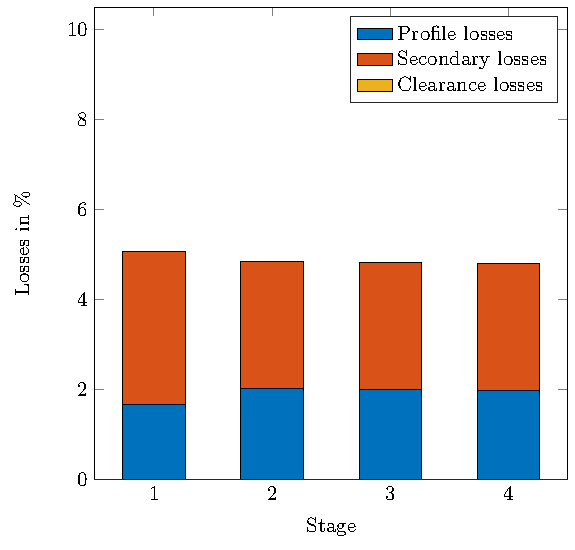
\includegraphics[height=5.25cm]{fig/stator_losses.pdf} }}%
    \subfloat{{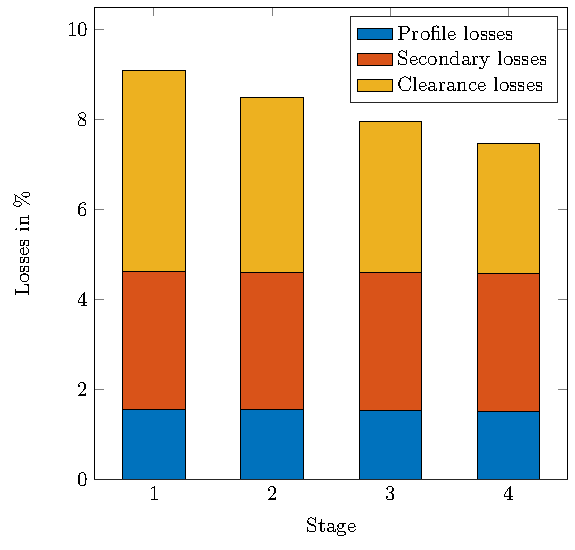
\includegraphics[height=5.25cm]{fig/rotor_losses.pdf} }}%
\end{figure}
\end{frame}


\begin{frame}[t]{The results - Profile losses along the span}
\begin{center}
Losses of the four stages for the stators and the rotors.
\end{center}
\vspace{-0.4cm}
\begin{figure}%
    \centering
    \subfloat{{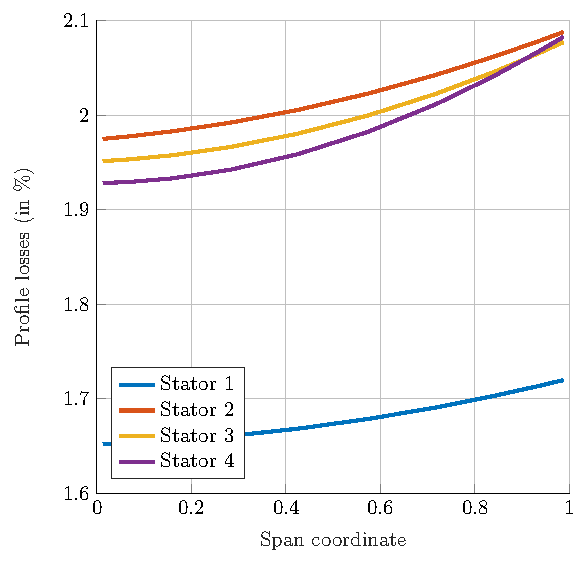
\includegraphics[height=5.25cm]{fig/stator_losses_span.pdf} }}%
    \subfloat{{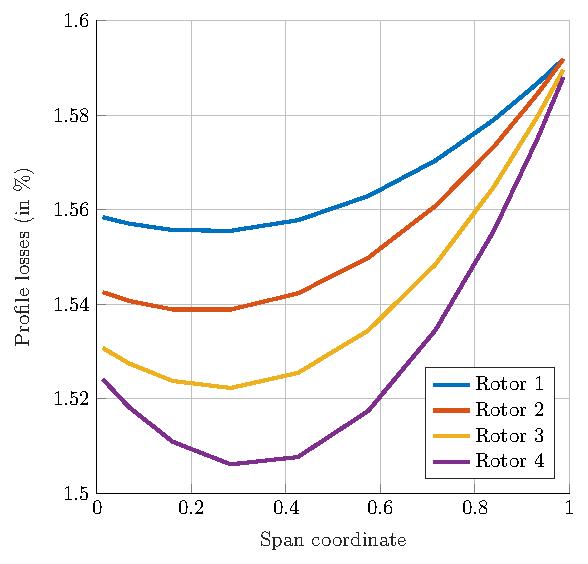
\includegraphics[height=5.25cm]{fig/rotor_losses_span.pdf} }}%
\end{figure}
\end{frame}


\begin{frame}[t]{The results - TS transformation}
\begin{center}
Representation of the stages in the T-S plane and the comparison with the liquid vapour curve.
\end{center}
\vspace{-0.8cm}
\begin{figure}%
    \centering
    \subfloat{{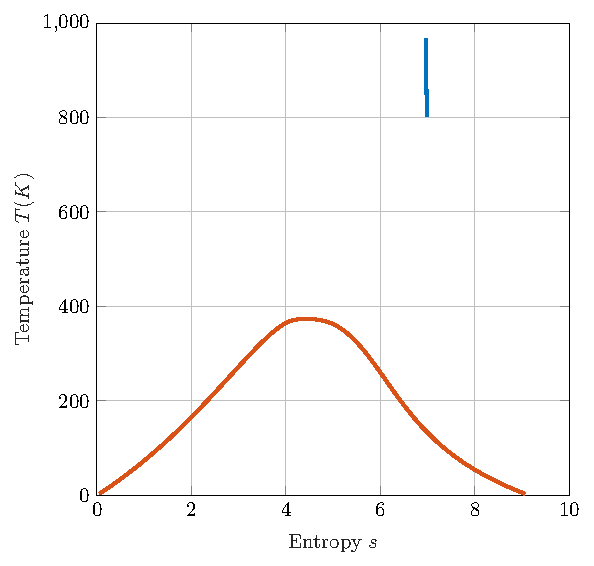
\includegraphics[height=5.25cm]{fig/machine_ts_global.pdf} }}%
    \subfloat{{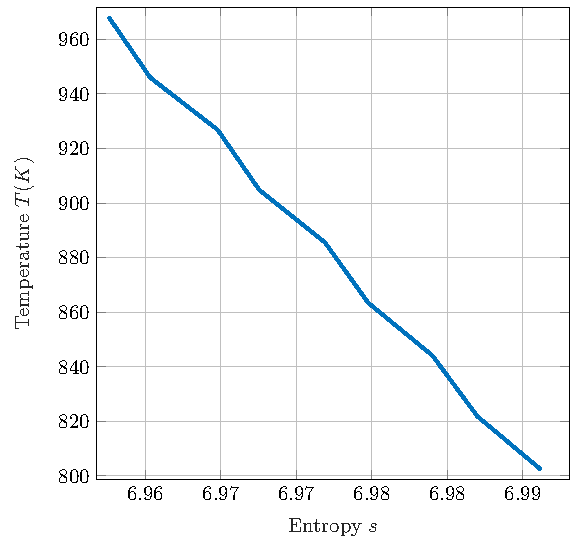
\includegraphics[height=5.25cm]{fig/machine_ts_local.pdf} }}%
\end{figure}
\end{frame}


\begin{frame}[t]{The results -  The temperature}

\myspaceneg
\myspaceneg
\begin{center}
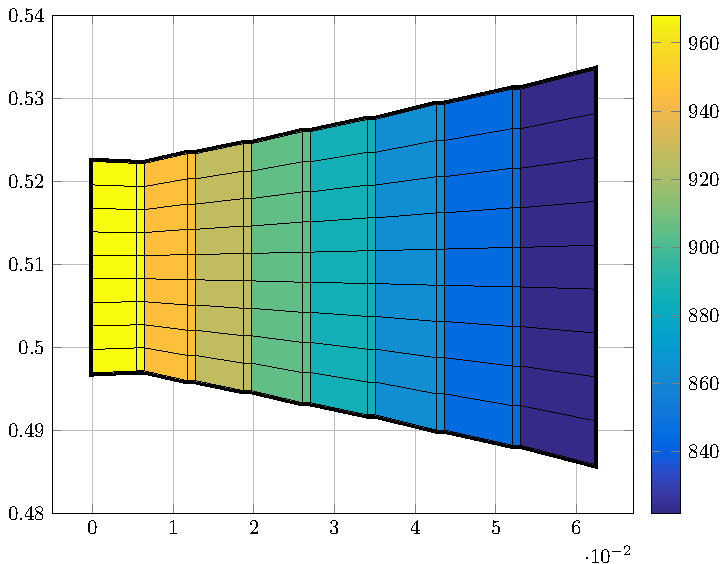
\includegraphics[height=7cm]{fig/machine_T.pdf} 
\end{center}
\end{frame}

\begin{frame}[t]{The results -  The pressure}

\myspaceneg
\myspaceneg
\begin{center}
 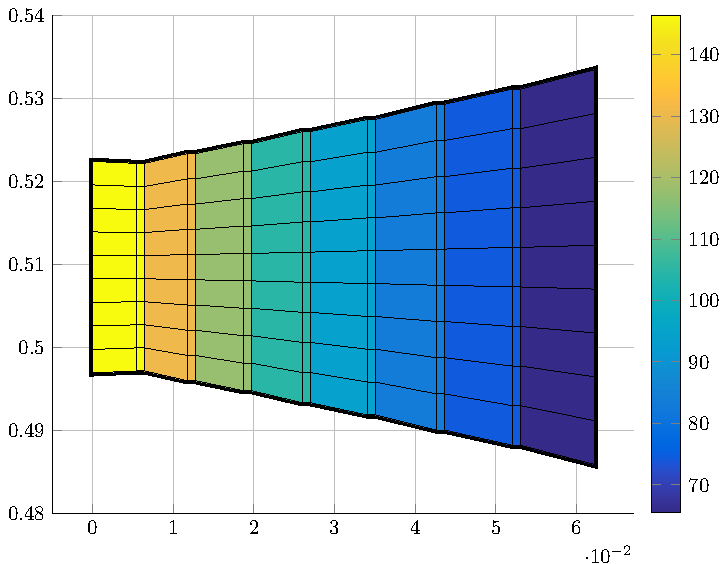
\includegraphics[height=7cm]{fig/machine_p.pdf}
 \end{center} 
\end{frame}

\begin{frame}[t]{The results -  The density}

\myspaceneg
\myspaceneg
\begin{center}
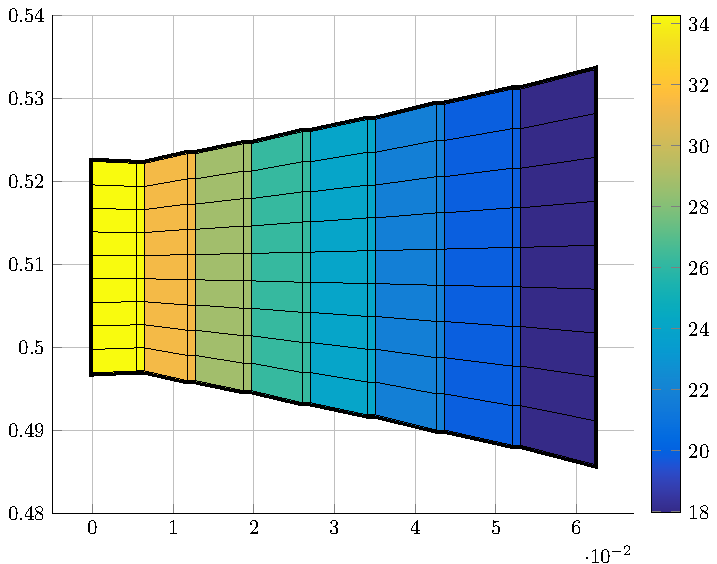
\includegraphics[height=7cm]{fig/machine_rho.pdf} 
\end{center}
\end{frame}


\begin{frame}[t]{The results -  The cascade}

\myspaceneg
\myspaceneg
\begin{center}
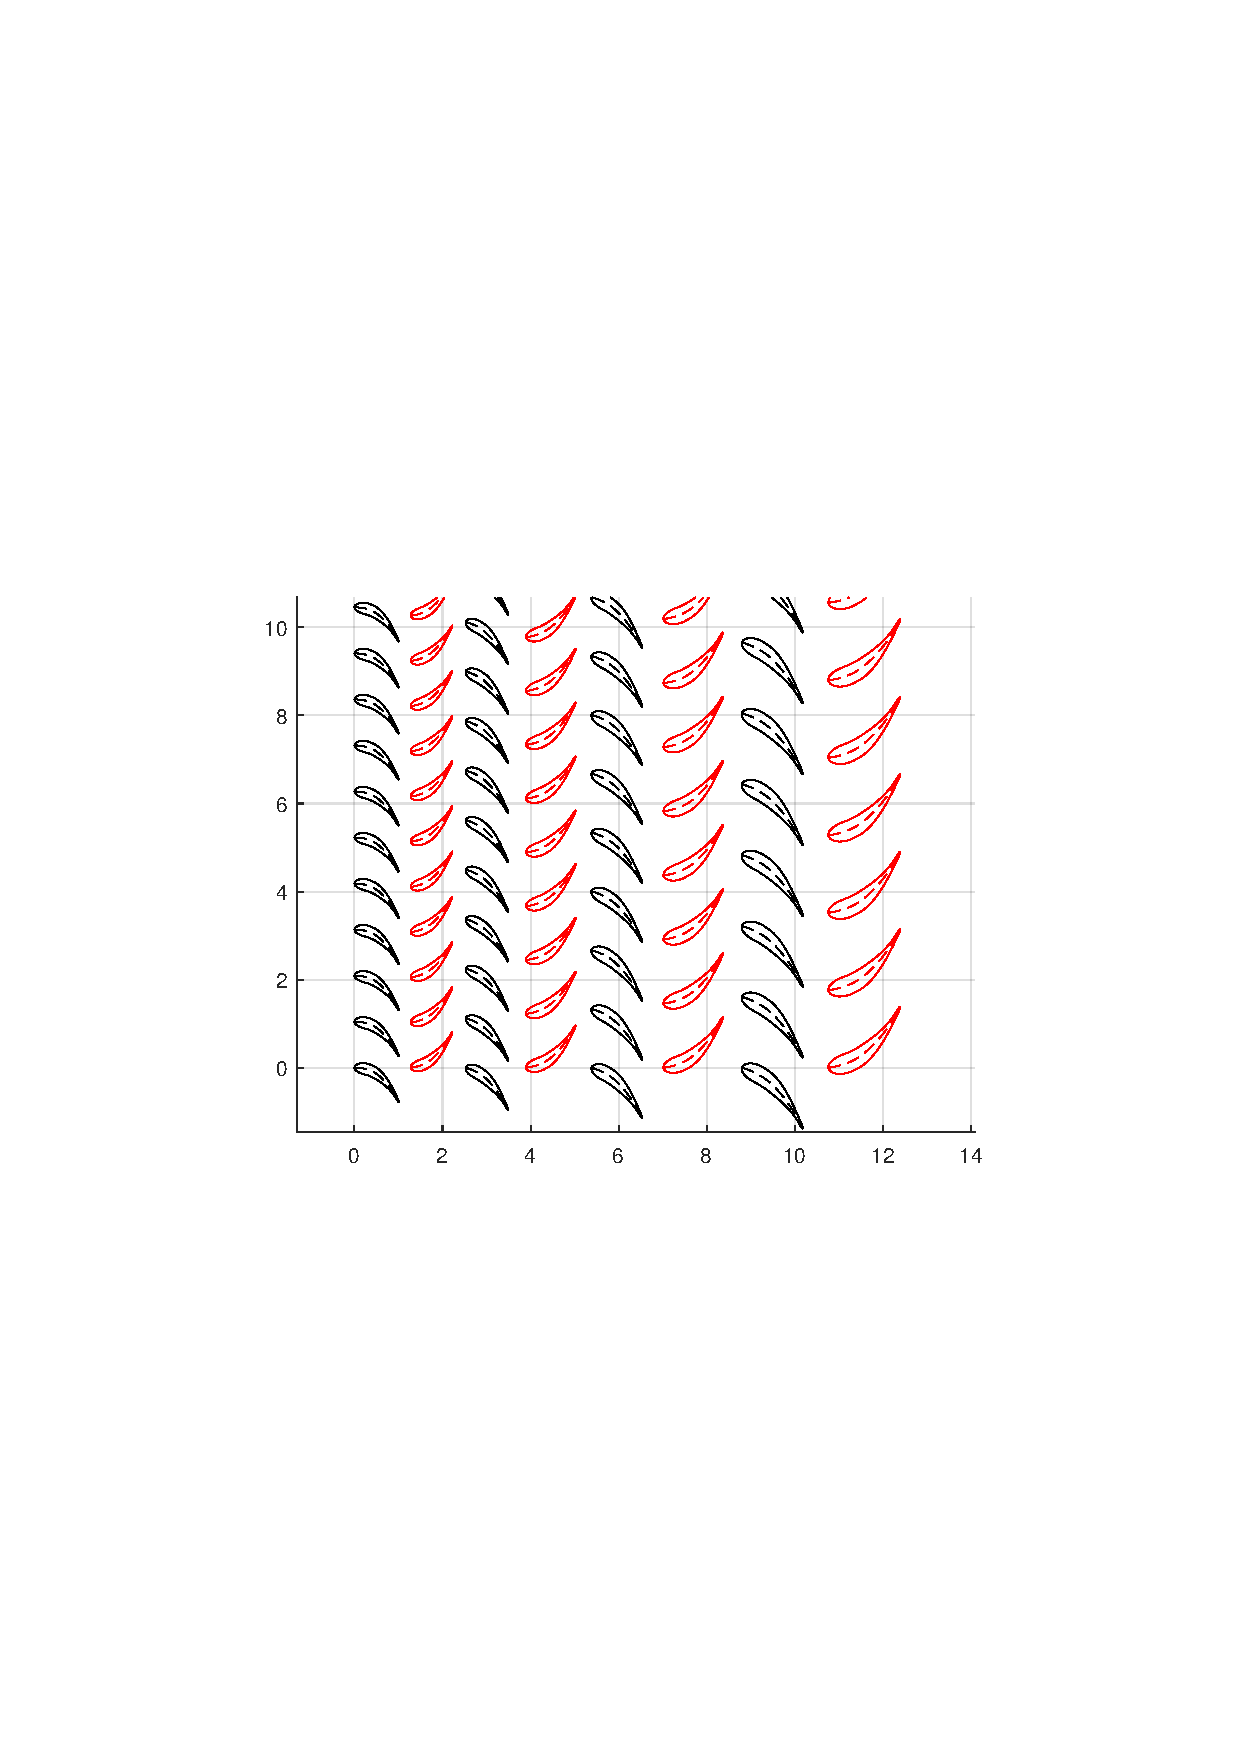
\includegraphics[height=7cm]{fig/blades.pdf} 
\end{center}
\end{frame}



\begin{frame}
\vspace{-0.2cm}

\begin{table}[]
\centering
\caption{Stator properties}
\vspace{-0.3cm}
\scalebox{0.8}{
\begin{tabular}{|l|c|c|c|c|c|c|}
\hline
Stage & Blades & Solidity & $\beta$ & Blade h.($m$) & Inlet M & $C_p$ \\ \hline
1     & 156    & 1.219    & 1.121   & 0.025             & 0.194                     & 2524.1                     \\ \hline
2     & 131    & 1.217    & 1.124   & 0.027             & 0.463                    & 2480.5                     \\ \hline
3     & 110    & 1.223    & 1.130   & 0.033             & 0.473                     & 2437.8                     \\ \hline
4     & 91     & 1.220    & 1.136   & 0.039             & 0.484                     & 2395.9           \\ \hline           
\end{tabular}}
\end{table}

\vspace{-0.3cm}

\begin{table}[]
\centering
\caption{Rotor properties}
\vspace{-0.3cm}
\scalebox{0.8}{
\begin{tabular}{|l|c|c|c|c|c|c|}
\hline
Stage & Blades & Solidity & $\beta$ & Blade h.($m$) & Inlet $M_w$ & $C_p$  \\ \hline
1     & 143              & 1.223    & 1.110   & 0.025         & 0.198       & 2501.2 \\ \hline
2     & 119              & 1.214    & 1.114   & 0.030         & 0.202       & 2458.2 \\ \hline
3     & 99               & 1.214    & 1.119   & 0.036         & 0.207       & 2415.8 \\ \hline
4     & 82               & 1.218    & 1.125   & 0.043         & 0.212       & 2374.3 \\ \hline
\end{tabular}}
\end{table}

\vspace{-0.5cm}

\begin{table}[]
\centering
\caption{Stage properties}
\vspace{-0.3cm}
\scalebox{0.8}{
\begin{tabular}{|l|c|c|c|c|}
\hline
Stage          & $\chi$     & $\eta_{TT}$    & $\beta$        & $\beta_{TT}$   \\ \hline
1              & 0.461      & 0.927          & 1.244          & 1.240          \\ \hline
2              & 0.465      & 0.930          & 1.252          & 1.251          \\ \hline
3              & 0.465      & 0.933          & 1.264          & 1.263          \\ \hline
4              & 0.465      & 0.936          & 1.278          & 1.276          \\ \hline
\textbf{Total} & \textbf{-} & \textbf{0.936} & \textbf{2.518} & \textbf{2.500} \\ \hline
\end{tabular}}
\end{table}
\end{frame}




\begin{frame}[t]{Further develops}
\begin{itemize}
\item Compare constant angle with other methodologies;
\item Iterate to guarantee the required work along the span;
\item Different solidity for the rotor and the stator;
\item Variable $\chi$ with stages (lower in the first stages);
\item Off-design performances;
\item Mechanical analysis
	\begin{itemize}
		\item Optimize rotor internal diameter.
		\item Vibration analysis and natural frequencies.
	\end{itemize}
\item Apply more refined losses correlation.
\item Clearance design;
\item Cost/performance comparison between 3000 and 6000 rpm.
\end{itemize}
\end{frame}


\begin{frame}
\end{frame}






















%
%
%
%
%\begin{frame}[t]{What is this?}
%\begin{itemize}
%\item Beamer is a \LaTeX{} class that allows you to create presentations
%\item The project home page is http://latex-beamer.sourceforge.net/
%\item Beamer contains several themes, but they are a bit ugly
%  \begin{itemize}
%  \item But with a lot of useful features, such as navigation bars, outlines,
%        etc.
%  \end{itemize}
%\item Torino is a pretty theme
%  \begin{itemize}
%  \item With a lot of useless -- but pretty -- features
%  \item But without some useful features
%  \item Well suited for short talks, for longer talks you should use themes
%        with navigation bars
%  \end{itemize}
%\item Why the name?
%  \begin{itemize}
%  \item Other themes are named after locations of Universities or conferences
%  \item Torino (Turin) is the location of Politecnico di Torino, my university
%  \end{itemize}
%\end{itemize}
%\end{frame}
%
%\begin{frame}[t,fragile]{How to use the theme}
%\begin{itemize}
%\item Install Beamer
%  \begin{itemize}
%  \item Some distros have a \verb!latex-beamer! package
%  \end{itemize}
%\item Read the Beamer documentation
%  \begin{itemize}
%  \item \verb!/usr/share/doc/latex-beamer/beameruserguide.pdf.gz! if you are
%        using Debian
%  \item \verb!doc/beameruserguide.pdf! in the source package
%  \end{itemize}
%\item Install the theme
%  \begin{itemize}
%  \item \verb!mkdir -p ~/texmf/tex/latex/beamer!\\
%  \item \verb!cp *.sty ~/texmf/tex/latex/beamer!
%  \end{itemize}
%\item Read the example files
%  \begin{itemize}
%  \item \verb!chameleon.tex!: green theme, watermark and circles for bullet
%        lists
%  \item \verb!nouvelle.tex!: green and red theme, watermark and squares for
%        bullet lists
%  \item \verb!freewilly.tex!: blue theme, a logo and squares for bullet lists
%  \end{itemize}
%\end{itemize}
%\end{frame}
%
%\begin{frame}[t,fragile]{Theme files}
%\begin{itemize}
%\item Themes are composed by sub-themes for single features
%\item Inner themes define how the title page, the bullet lists, margins,
%      etc. work
%  \begin{itemize}
%    \item \verb!beamerinnerthemefancy.sty!
%  \end{itemize}
%\item Outer themes define how headers and footers look like
%  \begin{itemize}
%    \item \verb!beamerouterthemedecolines.sty!
%  \end{itemize}
%\item Color themes define the colors to be used in outer and inner themes
%  \begin{itemize}
%    \item \verb!beamercolorthemechameleon.sty!: green footers and headers
%    \item \verb!beamercolorthemenouvelle.sty!: green footers, red headers and
%          and frame title
%    \item \verb!beamercolorthemefreewilly.sty!: blue footers, headers and
%          frame title
%  \end{itemize}
%\item Global themes just include inner, outer and color themes
%  \begin{itemize}
%    \item \verb!beamerthemeTorino.sty!
%  \end{itemize}
%\end{itemize}
%\end{frame}
%
%\begin{frame}[t,fragile]{Configuring the theme}
%\begin{itemize}
%\item Beamer themes can be configured with options between \verb![! and
%      \verb!]!
%  \begin{itemize}
%  \item \verb!\usetheme[option1 = value, option2 = value]{Torino}!
%  \end{itemize}
%\item If you do not specify any option, you get
%  \begin{itemize}
%  \item Simple title page
%  \item No watermark or logo
%  \item Chameleon (green) color theme
%  \item Squares for bullet lists
%  \end{itemize}
%\item Color themes can be changed with \verb!\usecolortheme!
%  \begin{itemize}
%  \item \verb!\usecolortheme{nouvelle}!: green and red
%  \item \verb!\usecolortheme{freewilly}!: blue
%  \end{itemize}
%\item A logo, shown in the upper right corner, can be choosen with the
%      \verb!\logo! command
%  \begin{itemize}
%  \item \verb!\logo{\includegraphics[height=50px]{logo-image}}!
%  \end{itemize}
%\end{itemize}
%\end{frame}
%
%\begin{frame}[t,fragile]{Alternative title page}
%\begin{itemize}
%\item A fancy title page can be enabled with the \verb!alternativetitlepage!
%      option
%\item You can put a logo in the title page, just pass the file name using the
%      \verb!titlepagelogo! option
%\item Remember to use a plain and top-aligned frame when using alternative title
%      pages:\\
%      \vskip1ex
%      \verb!\begin{frame}[t,plain]!\\
%      \verb!\titlepage!\\
%      \verb!\end{frame}!
%\end{itemize}
%\end{frame}
%
%\begin{frame}[t,fragile]{Watermark}
%\begin{itemize}
%\item A watermark can be shown in the bottom right corner of frames
%\item Use the \verb!watermark! option to set name of the image file
%\item The \verb!watermarkheight! option specifies the height of the watermark
%      image
%\item It's a good idea to have a big image and shrink it, so it looks good
%      when the slide is full screen
%\item If the image height in the slide is not the same as the original one,
%      you have to use the \verb!watermarkheightmult! option
%  \begin{itemize}
%  \item For example, if the image is 400 pixel tall but you want it to
%        occupy only 100 pixels, use
%        \verb![watermarkheight=100px, watermarkheightmult=4]!
%  \item It's ugly but I don't know how to fix it
%  \end{itemize}
%\end{itemize}
%\end{frame}
%
%\watermarkoff
%\begin{frame}[t,fragile]{Disabling the watermark}
%\begin{itemize}
%\item You may want to disable the watermark on some frames
%  \begin{itemize}
%  \item For example, an image could partially cover the watermark, with ugly
%        results
%  \end{itemize}
%\item The \verb!\watermarkoff! command can be used to disable the watermark
%      in the following frames
%\item The \verb!\watermarkon! command restores the watermark in the following
%      frames
%\item If you did not specify a watermark, nothing happens
%\vskip5ex
%\item \verb!\watermarkoff! was used for this frame
%\end{itemize}
%\end{frame}
%\watermarkon
%
%\begin{frame}[t,fragile]{Other options}
%\begin{itemize}
%\item The \verb!pageofpages! option defines the string between the current
%      page number and the total page count
%  \begin{itemize}
%  \item The default is ``/''
%  \item The example files set \verb!pageofpages! to ``of''
%  \end{itemize}
%\item The \verb!bullet! option can be used to choose the symbol used in
%      bullet lists
%  \begin{itemize}
%  \item \verb!square!: A filled square
%        ({\usebeamercolor[fg]{item}\tiny\raise0.2ex\hbox{$\blacksquare$}}) for
%        first and third level items, an empty square
%        ({\usebeamercolor[fg]{item}\tiny\raise0.2ex\hbox{$\square$}}) for
%        second level items
%  \item \verb!circle!: A filled circle ({\usebeamercolor[fg]{item}$\bullet$})
%        for first and third level items, an empty circle
%        ({\usebeamercolor[fg]{item}$\circ$}) for second level items
%  \item The default value is \verb!square!
%  \end{itemize}
%\item If the \verb!titleline! option is set to \verb!true!, a horizontal line
%      is drawn below the title
%\end{itemize}
%\end{frame}
\end{document}